\chapter{Methodology for The Quantitative Valuation of Flexibility Solutions}
\chaptermark{Methodology}
\label{ch:methodology}
\textit{This chapter presents the methodology for quantifying the value of flexibility solutions. A modular approach is adopted to overcome the complexity from multi-dimensional market-technology contexts. A total of 6 modules are developed, being categorized into two groups, i.e. market- and technology- based modules. We first introduce each of the modules and then explain how these modules are organized within an optimization.}

\section{Modular approach to build valuation models}
As discussed in Chapter \ref{ch:introduction}, the quantitative work of this thesis aims at determining the market size and profitability of different flexibility solutions in various power market jurisdictions. By combing methodologies of other similar works reviewed in Chapter \ref{ch:LitRev} and our own analytical frameworks established in Chapter \ref{ch:market}, we develop a techno-economic model for the quantitative analysis. 

Since there are structural differences existing between technologies and between markets as we have seen in previous chapters, the model needs to be implemented in several modes. For instance, for $m$ technologies in $n$ market regimes, a total of $m \times n$ modes is required. In order to avoid redundancy and make the model easier to reuse and maintain in the future, we adopt a modular approach, breaking up the model into several modules with each module having dependencies on either technology or market. Using the same example, each module needs either $m$ or $n$ modes. The modular approach does not reduce the complexity of the problem, but renders the model more structurally organized.

Table \ref{tb:modules} offers an overview of all the modules and their inputs and outputs. The working flow of the model is illustrated by Figure \ref{fig:model-flow}. It should be noted for market-based modules there are two modes, i.e. using actual price-volume data  as input or using simulated price-volume signals as input. The rationale of implementing these two modes will be discussed later in Section \ref{sec:market-simulation}. %The merits and limitations respectively for these two modes have been discussed in Chapter \ref{ch:LitRev}

\begin{table}
	\footnotesize
	\centering
		\begin{tabular}{L{1.2cm} L{3.3 cm}  L{4.5 cm} L{3cm} }
			\hline %\hline
			\textbf{Section} &\textbf{Module name} & \textbf{Input} & \textbf{Output} %& \textbf{Parameters}
			\\
			\hline %\hline
			&&&\\
			\multicolumn{4}{l}{\textbf{Market-based modules}}\\%\hline
			\ref{sec:revenue} & Revenue & Price signals; Frequency control signals; Sets of targeted marketplaces & Matrix of coefficients for revenue calculation
			\\
			&&&\\%\hline
			\ref{sec:market-simulation} &Market simulation & Generation time-series by fuel type; Consumption time-series & Price and volume signals \\
			&&&\\%\hline
			\ref{sec:market-constraints} & Market constraints & Volume signals & Constraints for optimization\\
			%\hline
			\hline
			&&&\\
			\multicolumn{4}{l}{\textbf{Technology-based modules}} \\
			%\hline
			\ref{sec:cost} &Cost& Investment cost; Designed life time; Operating life time; System state & Matrix of coefficients for cost calculation %& None
			\\
			&&&\\%\hline
			\ref{sec:tech-simulation-module}&Technology simulation & Efficiencies of charge, discharge and storage; Maximum charge, discharge rates; Energy-to-power ration& Matrix of coefficients to determine system states %& 3
			\\
			&&&\\%\hline
			\ref{sec:tech-constraints} &Technology constraints & System size, system state & Constraints for optimization
			\\
			 \hline
		\end{tabular}
	\caption{List of modules}\label{tb:modules}
\end{table}

\begin{figure}[h!]
	\centering
	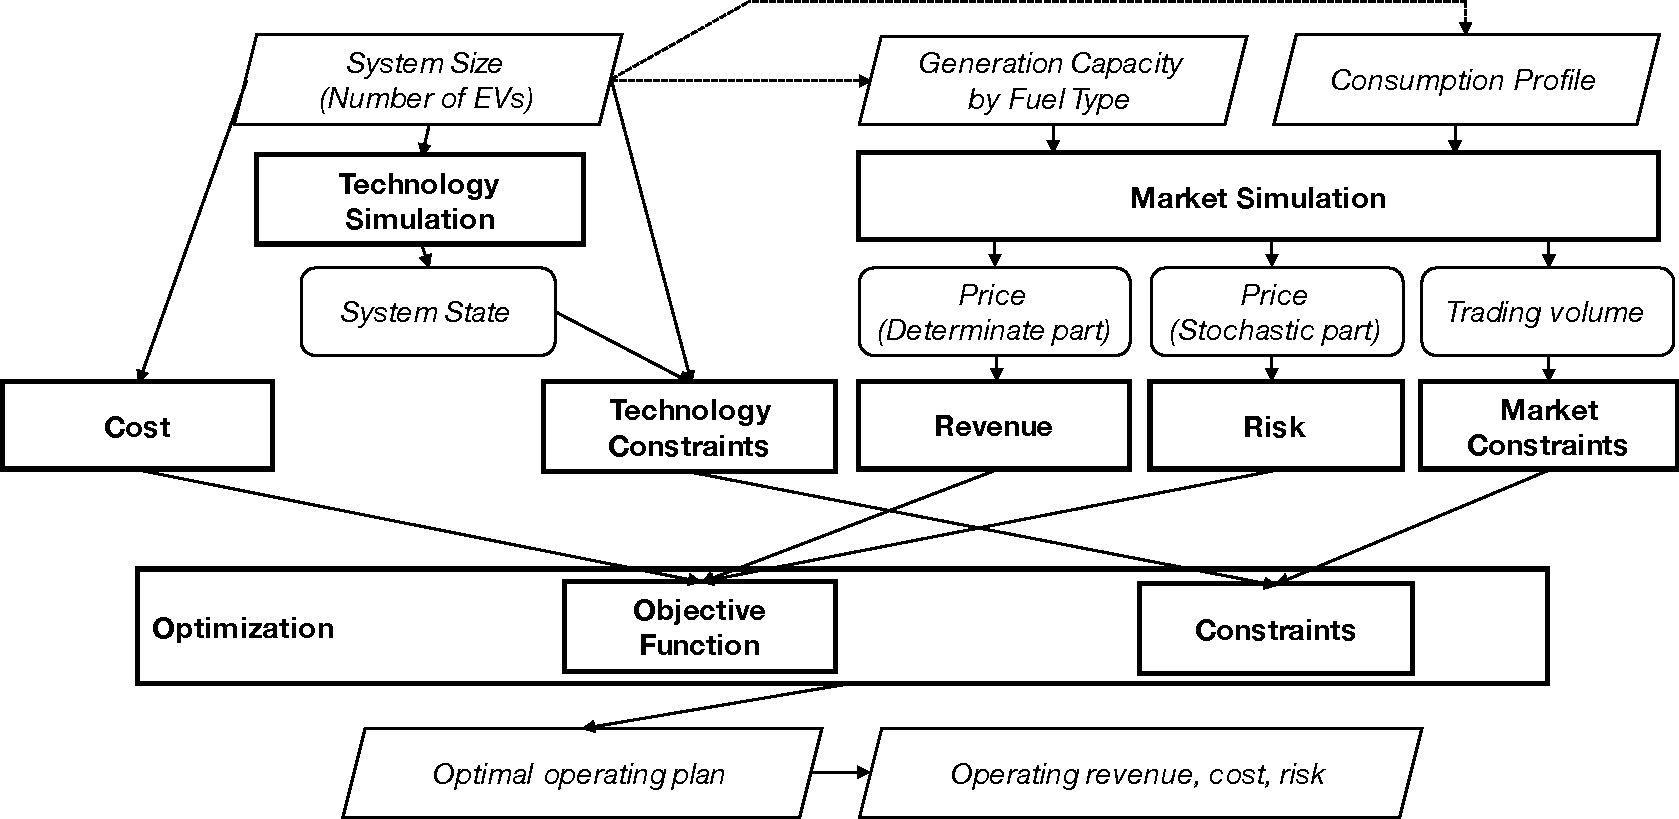
\includegraphics[width=0.95\linewidth]{Figures/ModelFlow}
	\caption{Flow chart of the techno-economic model}
	\label{fig:model-flow}
\end{figure}

Using this model, we can quantify the revenue and cost associated with the deployment of a given flexibility solution in a selected market and thus evaluate the profitability with any given scales of flexibility system in the power market. By taking into account market constraints including liquidity, marginal revenue with respect to system scale will drop when liquidity becomes scarce. This allows us to derive the maximum revenue potential in a market. Furthermore, impacts of renewable penetration and cost reduction that are raised in our initial research questions can be assessed since the share of renewable resources in generation mix and the cost parameters of flexibility systems are all made to be variables of the model.

\section{Market-based modules}

\subsection{Revenue module}
\label{sec:revenue}
As determined in the scope, we only quantify explicit revenues from arbitraging in energy markets and providing frequency control services in ancillary service markets in this thesis.

In each business case, trading can be performed in one, or more than one marketplace%, namely multitasking (referring to Section \ref{sec:lit-stacking})
. By denoting the set of selected marketplaces for energy arbitrage as $\mathbb{I}$ and index each marketplace as $i$, we can represent each of $I$ selected marketplaces as:

\begin{equation}
\label{eq:set-I}
	i \in \mathbb{I} = \{1,2,\dots,I\}
\end{equation}
where a marketplace $i$ could refer to day-ahead market or intra-day market or others; see Section \ref{sec:market-energy}

Applying the same exercise for frequency control services, we have the selected marketplaces in ancillary service markets denoted as:

\begin{equation}
\label{eq:set-J}
j \in \mathbb{J} = \{1,2,\dots,J\}
\end{equation}
where a marketplace $j$ could be the marketplace for PCR or SCR or others, referring to Section \ref{sec:market-as}.

For energy arbitrage, we need to determine at each time step $t$ in a certain marketplace $i$, the amount of energy to sell, denoted as $e^+_{t,i}$ in MWh, and the amount of energy to buy, denoted as $e^-_{t,i}$ also in MWh. The price signal at that marketplace is indicated as $\pi_{t,i}$ in USD/MWh\footnote{Other currencies used in certain markets, e.g. AUD in Australia's NEM, are convert to USD based on currency exchanged rates. Details will be provided in Section \ref{sec:data-parameter}.}.

In frequency control service, what is to be decided by the operator of flexibility resources is the amount of capacity offered in a certain marketplace $j$ at each time step $t$, denoted as $c_{t,j}$ in MW, the price of which is denoted as $\psi_{t,j}$ in USD/MW. The amount of energy delivered for frequency control services is determined upon request of system operator via the control signal. We represent the control signal for frequency control service in a marketplace $j$ at each time step $t$ as a ratio between the required energy and committed capacity, denoted as $\delta_{t,j}$ in MWh/MW. The price for the energy delivery is denoted as $\phi_{t,j}$ in USD/MWh. As introduced in Section \ref{sec:market-as}, in some market regimes, the performance will be considered in payment for frequency control service. Since evaluating performance could be a complex manner, we make some assumptions in specific cases and reflect the performance payment in the price signal $\phi_{t,j}$.

Thereby, we can finally calculate the total revenue $R$ from all marketplaces over a period of time $\mathbb{T}$ ($t \in \mathbb{T} = \{1,2,\dots, T\}$) as:

\begin{equation}
\label{eq:module-revenue}
R =  \sum_{t}^{t \in \mathbb{T}} R_t = \sum_{t}^{t \in \mathbb{T}} \left( \sum_{i}^{i \in \mathbb{I}}  \pi_{t,i} (e_{t,i}^{+} - e_{t,i}^{-})  + \sum_{j}^{j \in \mathbb{J}} (\phi_{t,j} \delta_{t,j} + \psi_{t,j}) c_{t,j} \right)
\end{equation}

In this equation, $e^+_{t,i}$, $e^-_{t,i}$ and $c_{t,j}$ are decision variables of the optimization problem to find a optimal operating plan. $e^+_{t,i}$, $e^-_{t,i}$ and $c_{t,j}$ are all non-negative values, i.e.:

\begin{equation*}
e^+_{t,i}, e^-_{t,i}, c_{t,i} \geq 0 ~~~ \forall t \in \mathbb{T},~ \forall i \in \mathbb{I},~ \forall j \in \mathbb{J}
\end{equation*}

Price signals $\pi_{t,i}$, $\phi_{t,j}$ and $\psi_{t,j}$ and frequency control signals $\delta_{t,j}$ are inputs of the revenue module. $\mathbb{I}$ and $\mathbb{J}$ are determined according to the business case to be studied. For example, we can set $\mathbb{I} = \{1\}$ and $ \mathbb{J}=\emptyset$ in order to value arbitrage in day-ahead energy market. 

%If there are multiple elements in $I \cup J$, it means the flexibility resource can be reallocated to make offers to different market segments, i.e. performing multitasking. These cases need to be carefully managed to comply with actual market rules. Detailed treatments regarding multitasking are illustrated in section \ref{sec:special}.

%The ratios $\delta_t$ are computed based on the real control signal when data is available, or otherwise using system average ratios between total activated energy ($\hat{e}_t^{r,j}$) and the total reserve ($\hat{e}_t^{r,j}$) at each time step.

%\begin{equation*}
%\delta_t^j = \frac{\hat{e}_t^{r,j}}{\hat{r}_t^j}
%\end{equation*}

%Price signals, $\pi_t^{e,i}$, $\pi_t^{r,j}$ and $\pi_t^{e,j}$, are inputs for the revenue module and may be retrieved either directly from historical data or from the outputs of market simulation module described in Section \ref{sec:market-simulation}.

For the ease of implementation, we re-formulate Equation \eqref{eq:module-revenue} as:

\begin{equation}
\label{eq:revnue-matrix}
R = \mathcal{R} \cdot X 
\end{equation}
where $X$ is the vector for all decision variables. %For certain sets of marketplaces $\mathbb{I} = \{1,2,\dots,I\}$ and $\mathbb{J} = \{1,2,\dots,J\}$,
With $i \in \mathbb{I} = \{1,2,\dots,I\}$,
$j \in \mathbb{J} = \{1,2,\dots,J\}$ and
$t \in \mathbb{T} = \{1,2,\dots,T\}$, $X$ can be derived by following the steps:

\begin{itemize}
	\item Formulating the time-series of energy to be sold, energy to be bought and reserve capacity in each marketplace into vectors:
	\begin{equation}
	\label{eq:Ei-Ei-Cj}
	E^+_{i} = 
	\begin{bmatrix}
	e^+_{1,i}\\e^+_{2,i}\\\vdots\\e^+_{T,i}
	\end{bmatrix} ~~~
	E^-_{i} = 
	\begin{bmatrix}
	e^-_{1,i}\\e^-_{2,i}\\\vdots\\e^-_{T,i}
	\end{bmatrix} ~~~
	C_{j} = 
	\begin{bmatrix}
	c_{1,j}\\c_{2,j}\\\vdots\\c_{T,j}
	\end{bmatrix} ~~~
	\end{equation}
	
	\item Connecting the vectors for each marketplace together:
	\begin{equation}
	E^+ = 
	\begin{bmatrix}
	E^+_{1}\\ \vdots \\ E^+_{i}\\ \vdots\\E^+_{I}
	\end{bmatrix} ~~~
	E^- = 
	\begin{bmatrix}
	E^-_{1}\\ \vdots \\ E^-_{i}\\ \vdots\\E^-_{I}
	\end{bmatrix} ~~~
	C = 
	\begin{bmatrix}
	C_{1}\\ \vdots \\ C_{i}\\ \vdots\\C_{I}
	\end{bmatrix} ~~~
	\end{equation}
	
	\item Finally connecting all vectors to obtain X as:
	
	\begin{equation}
	\label{eq:decision-variable-1}
	X =
	\begin{bmatrix}
	E^+ \\ E^- \\ C
	\end{bmatrix}
	\end{equation}
\end{itemize}


Matrix $\mathcal{R}$ can be obtained by following similar steps:

\begin{itemize}
	\item Formulating the time-series of price signals in each marketplace into vectors:
	
	\begin{equation*}
	\Pi_{i} = 
	\begin{bmatrix}
	~\pi_{1,i}~~\pi_{2,i}~~\dots~~\pi_{T,i}~
	\end{bmatrix}
	\end{equation*}
	\begin{equation*}
	\Phi_{j} = 
	\begin{bmatrix}
	~\phi_{1,j}~~\phi_{2,j}~~\dots~~\phi_{T,j}~
	\end{bmatrix}
	\end{equation*}
	\begin{equation*}
	\Psi_{j} = 
	\begin{bmatrix}
	~\psi_{1,j}~~\psi_{2,j}~~\dots~~\psi_{T,j}~
	\end{bmatrix}
	\end{equation*}
	
	\item Connecting the vectors of price signals for each marketplace together:
	
	\begin{equation*}
	\Pi=
	\begin{bmatrix}
	~\Pi_{1}~|~&\dots~|~&\Pi_{i} ~|~&\dots~|~&\Pi_{I}~
	\end{bmatrix}
	\end{equation*}
	\begin{equation*}
	\Phi=
	\begin{bmatrix}
	~\Phi_{1}~|~&\dots~|~&\Phi_{j} ~|~&\dots~|~&\Phi_{J}~
	\end{bmatrix}
	\end{equation*}
	\begin{equation*}
	\Psi =
	\begin{bmatrix}
	~\Psi_{1}~|~&\dots~|~&\Psi_{j} ~|~&\dots~|~&\Psi_{J}~
	\end{bmatrix}
	\end{equation*}
	
	\item Creating a diagonal matrix using frequency control signals:
	
	\begin{equation}
	\label{eq:decision-f-revenue-end}
	\Delta = diag (
	\delta_{1,1}, \delta_{2,1},\dots , \delta_{T,1},\delta_{1,2},\delta_{2,2}, \dots,\delta_{T,2}, \dots, \delta_{T,J})
	\end{equation}
	
	\item Finally $\mathcal{R}$ is calculated as:
	
	\begin{equation}
	\label{eq:decision-f-revenue-1}
	\mathcal{R} =
	\begin{bmatrix}
	~\Pi~|~&-\Pi~|~&\Phi \cdot \Delta + \Psi~
	\end{bmatrix}
	\end{equation}
	
\end{itemize}
\subsubsection{Summary}
A high-level summary about the key information for revenue model is provided as listed below:
\begin{table}[h!]
	\begin{tabular}{L{0.95\textwidth}}
		\hline
		\textbf{Summary of revenue module} \\
		\hline
		\\
		\textbf{Decision variable:}  X\\
		\\
		\textbf{Input:} \\
		~~~Price signals: $\Pi$, $\Phi$, $\Psi$ \\
		~~~Frequency control signal: $\Delta$\\
		~~~Selected marketplaces: $\mathbb{I}$, $\mathbb{J}$\\
		\\
		\textbf{Output:} \\
		~~~Coefficient matrix: $\mathcal{R}$ \\
		\\
		\hline
	\end{tabular}
\end{table}

\subsection{Market simulation module}
\label{sec:market-simulation}
As discussed in Section \ref{sec:lit-price}, using historical data of price as input is a common exercise, which offers a pragmatic way to derive reference values that are valid in near future. This method is also adopted in this thesis to do valuation under current market conditions. However, using historical data as fixed input prevents us from understanding a long-term trend with potential changes, among which we are particularly interested in the impact of renewable penetration, i.e. increasing share of RES in generation mix. To overcome the limitation of using historical price signals, we developed this market simulation module for generating future price scenarios but only for valuation of energy arbitrage as discussed in Section \ref{sec:lit-price}.

In Chapter \ref{ch:LitRev}, we have illustrated that our questions are not perfectly answered in the literature. We are interested in both long-term price trends over a relative large scope of time as well as short-term price movement in high time resolution. In the literature, the former is usually evaluated using a deterministic merit-order model and the latter is often simulated using a stochastic SARIMA model, as discussed in Section \ref{sec:lit-price}. We combine these two approaches. In order to simulate prices in energy markets, we first use the merit-order model to get a determinant price signal in day-ahead market, denoted as $\tilde{\pi}$. The actual price signals, denoted as $\pi$, in day-ahead as well as in other energy markets, e.g. intra-day and real-time, are largely dependent on the merit-order price. Deviations may come from various factors and we tackle them purely in a statistical way by viewing them as stochastic processes and simulating them in the SARIMA model. We denote the stochastic part of the price as $\dot{\pi}$. Thereby, the output of market simulation model is the combination of output from merit-order model and SARIMA model, as shown below:

\begin{equation}
\pi = \tilde{\pi} + \dot{\pi}
\end{equation}

In actual implementation, the merit-order model and SARIMA model are first parameterized using historical data, see Figure \ref{fig:ms-parameterization}. 

Compared to other studies working on merit-order models, this thesis has a particular focus on flexibility so we categorize the capacity of generation into four classes considering their impacts on overall system flexibility. These four classes are non-dispatchable RES, inflexible, middle and peak generations. As discussed in Chapter \ref{ch:introduction}, RES generation is often taken out separately and compared to the consumption, to get the so-called residual load. The other three classes are obtained by running a algorithm that is originally developed in this thesis and is able to analyze power plants' level of flexibility. Using the classified generation, residual load as well as the historical price data, regressions are performed to determine the parameters of the merit-order model. 

Thereafter, we further compared the actual price data and the fitted price derived from the merit-order model. With the concern that regressions will eliminate the stochastic movement of price and reduce the price volatility which impact the value of arbitrage, we further parameterize a SARIMA model to re-capture the eliminated stochastic price movement. 

\begin{figure}[h!]
	\centering
	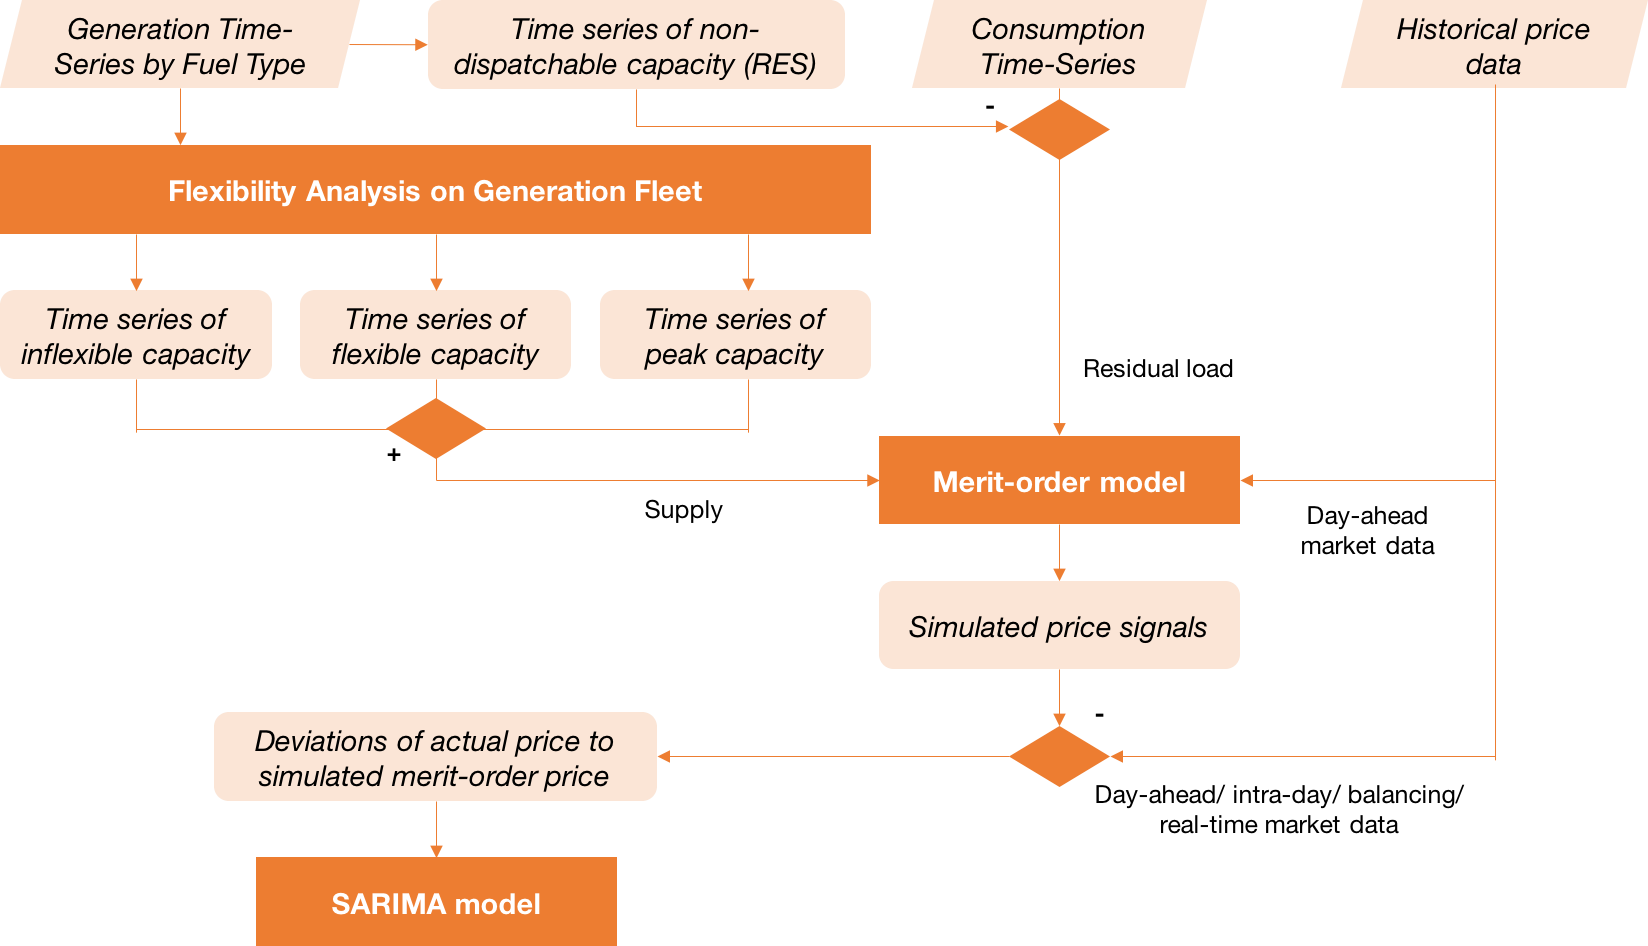
\includegraphics[width=0.95\linewidth]{Figures/MarketSimulationParameterization}
	\caption{Parameterization of the merit-order model and SARIMA model}
	\label{fig:ms-parameterization}
\end{figure}


\begin{figure}[h!]
	\centering
	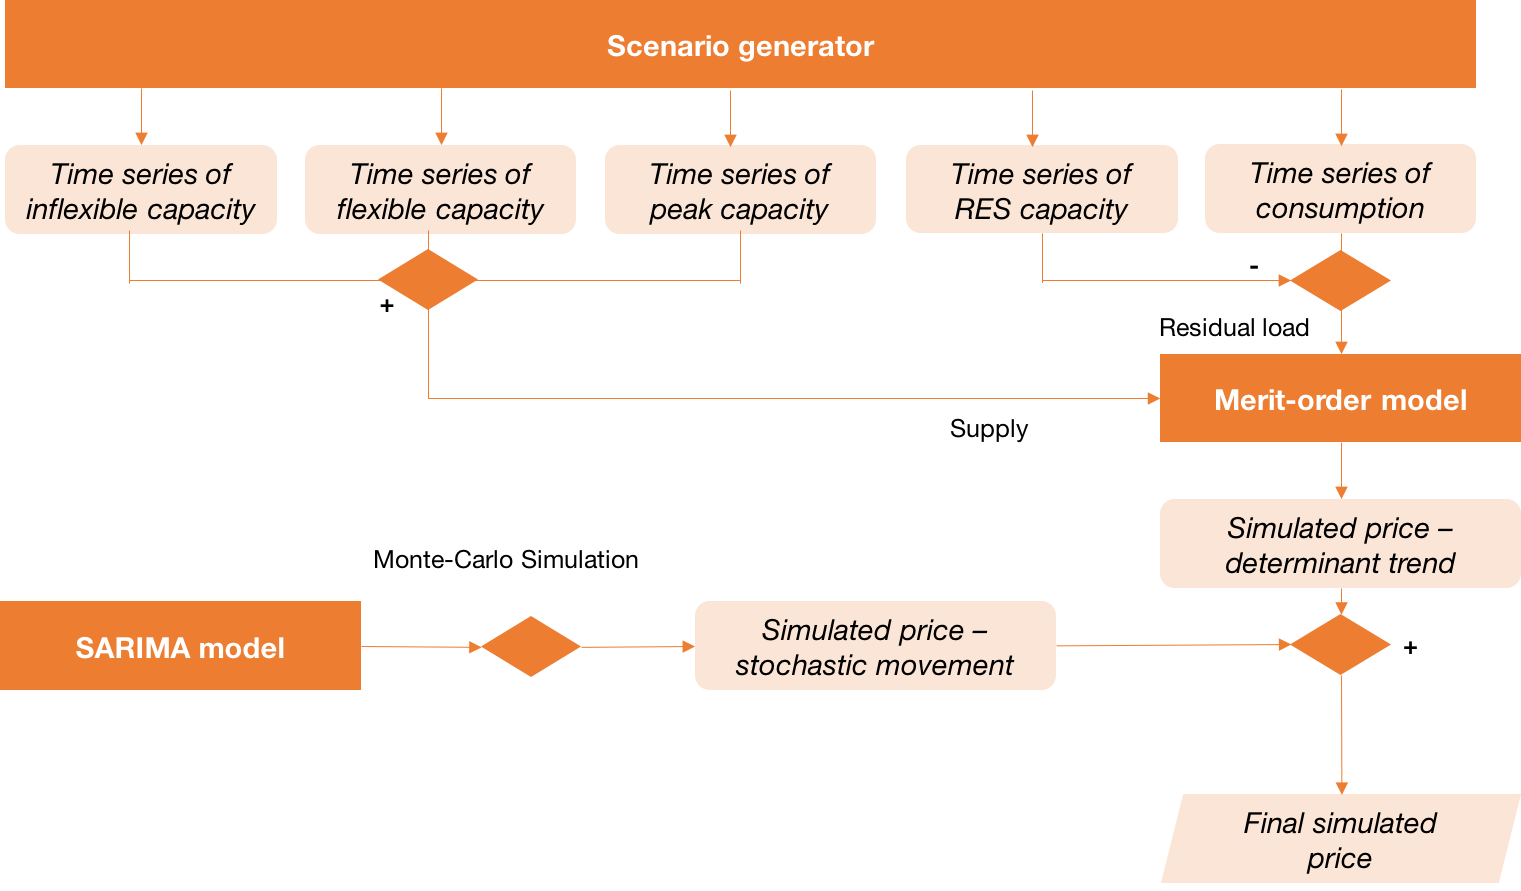
\includegraphics[width=0.95\linewidth]{Figures/MarketSimulationSimulation}
	\caption{Simulation of price using the merit-order model and SARIMA model based on given scenario}
	\label{fig:ms-simulation}
\end{figure}

With these two model, we can then simulate price signals for different scenarios where the time-series of supply and consumption are generated based on a given scenario (Figure \ref{fig:ms-simulation}). Details of these two sub-models together with the algorithm of flexibility analysis of generation fleet are introduced in the reminder of this section.
%Therefore, in this thesis, we customized a market model based on existing researches by re-focusing on factors that are most relevant to our research questions, and simplifying many other aspects of the power system and markets. Our market model is generally a statistic model built on observations of historical data, but a physical sub-model is incorporated as well to study the impacts of some relevant variables whose features are not well captured by empirical observations.

%The approach for market simulation differentiates between energy markets and reserve markets. 

\subsubsection{Flexibility analysis on  generation fleet}
In Chapter 1, we mentioned that increasing share of RES in total generation mix will raise the need for flexibility. Lack of flexibility will possibly lead to negative market prices, and high price volatility in wholesale energy markets. The mechanism behind these observations are modeled here by investigating the flexibility of different types of power plants. 

The flexibility of a power plant can be characterized by three key features \cite{AgoraEnergiewende2017}:

\begin{itemize}
	\item Overall bandwidth of operation: the range of output between minimum and maximum load;
	\item Ramp rate: the speed of adjusting output;
	\item Start-up time: the time required to attain stable operation from standstill, i.e. cold start.
\end{itemize}

A graphic illustration is provided by Figure \ref{fig:power-plant-flexibility}. 

\begin{figure}[h!]
	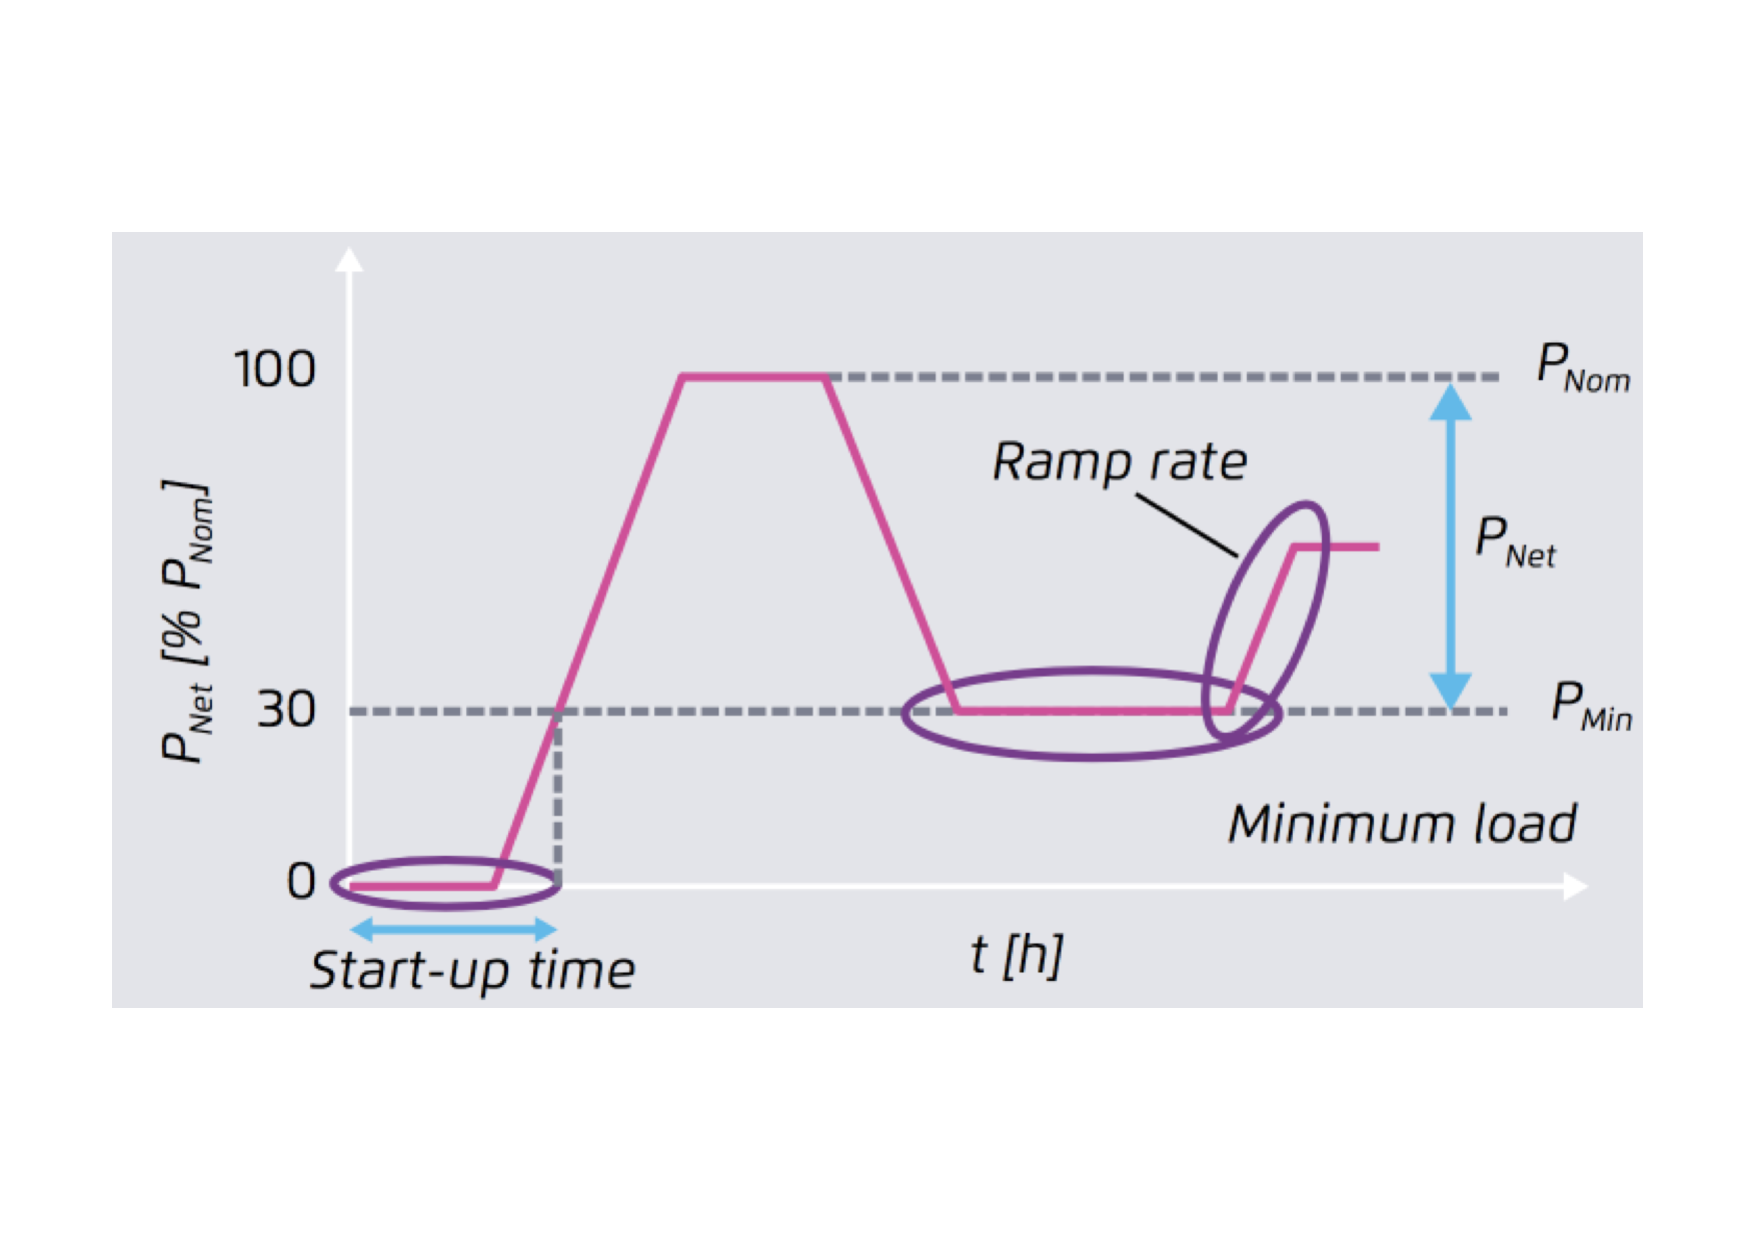
\includegraphics[width=0.95\linewidth]{Figures/PowerPlantFlexibility.pdf}
	\caption{Illustration of key flexibility parameters of a power plant\cite{AgoraEnergiewende2017}}	\label{fig:power-plant-flexibility}
\end{figure}

%https://www.researchgate.net/profile/Alejandro_Hoese
If a power plant can adjust its load from zero to nominal capacity within a time interval in the day-ahead market (typically 1 hour), it can be deemed to have unlimited flexibility in the day-ahead market. This applies to many types of generation technologies, such as hydro, electrochemical systems and gas turbines \cite{Muller2016,AgoraEnergiewende2017,Siemens,GE}. However, for power plants using steam turbines, e.g. coal, lignite and nuclear power plants, their ability to adjust output within short time interval is limited. For a steam-turbine power plant, a cold start (starting from standstill) may take up to 100 hours or at least 4 hours even with the state-of-the-art thermal power plants \cite{Muller2016} and the minimum operational load is about 25-60\% of its nominal capacity \cite{AgoraEnergiewende2017}. Therefore, in order to avoid cold starts that lead to long-time shutdown, steam-turbine power plants have to keep a minimum output, which leads to hard inflexibility. Furthermore, even within the overall bandwidth of operation, steam-turbine power plants may not be able to ramp to any given level of output due to relative slow ramp rate \cite{Muller2016}. Therefore, for those conventional power plants, their flexibility is bounded within a certain time interval. We refer to these power plants as \textit{flexibility-limited}.

In order to quantitatively model the effect of inflexibility, we need to quantify the amount of capacity by its level of flexibility. An algorithm is therefore developed. In the algorithm, we take the whole of all power plants with the same fuel type in a power system as the basic unit system, denoted as $f$. The overall generation fleet can be then viewed as a set of these unit systems, denoted as $\mathbb{F}$. For each $f \in \mathbb{F}$, if it belongs to the flexibility-limited generation as discussed above, we will run the procedure listed below and illustrated graphically by Figure \ref{fig:bounded-flexibility}:

\begin{figure}[h!]
	\label{fig:bounded-flexibility}
	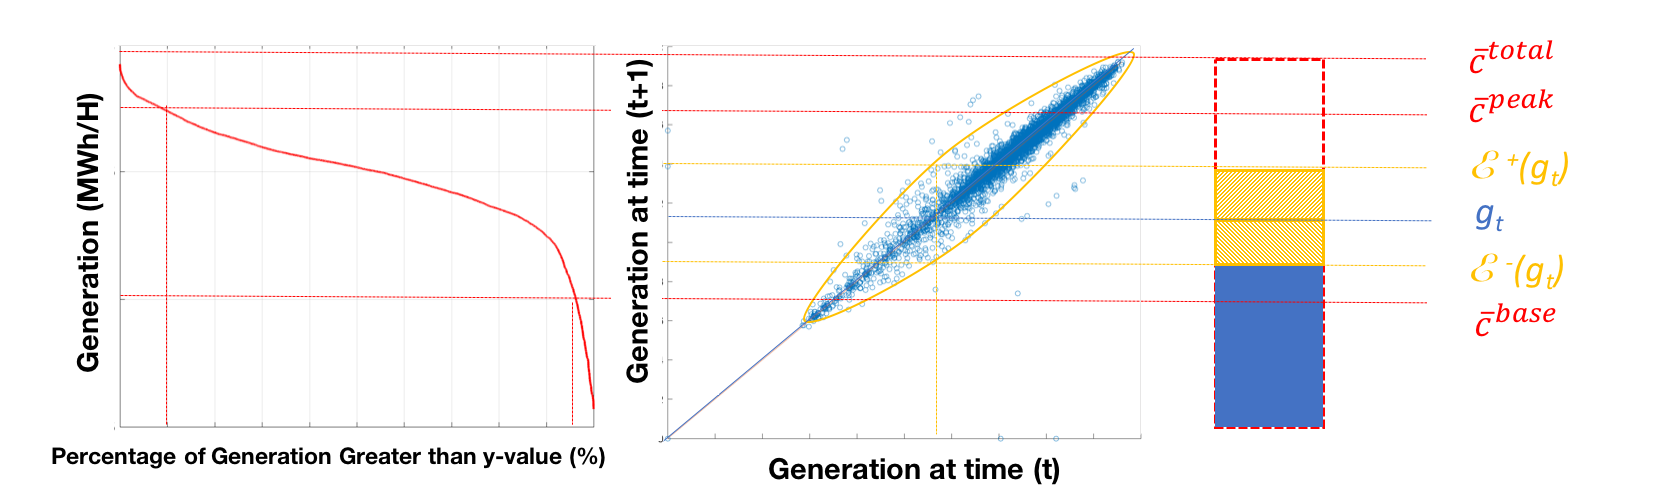
\includegraphics[width=1.05\linewidth]{Figures/BoundedFlexibility}
	\caption{Schematic illustration of determining bounded flexibility for limited flexible generations}
\end{figure}

\begin{enumerate}
	\item Make the duration curve using the generation data of a given fuel type $f$, e.g. generation of all coal-fired power plants in a power system, over a given period.
	
	\item From the duration curve, determine two time invariants, $\overline{c}_f^{\text{peak}}$ and $\overline{c}_f^{\text{base}}$. The term $\overline{c}_f^{\text{peak}}$ represents the capacity that is operated for only a small percentage (e.g. 10\%) of time so can be viewed as the capacity that would be only activated for peak hours (e.g. 2.4 hours per day with the percentage being 10\%), and $\overline{c}_f^{base}$ is the capacity operated for all time so represents the base load. However, since in the real world there are always data defects, we would set a threshold to exclude the outliers. 
	
	\item Compare the generation at each time time $t$, denoted as $g_{t,f}$, to the generation at next time step $t+1$, denoted as $g_{t+1,f}$. As analyzed previously, for flexibility-limited power plants, $g_{t+1,f}$ will be bounded within a certain range. Therefore, we determine the envelop lines of $g_{t+1,f}$ as functions of $g_{t,f}$. By denoting the upper envelop line as $\mathcal{E}_f^+(\cdot)$ and the lower envelop line as $\mathcal{E}_f^-(\cdot)$, we have:
	
	\begin{equation*}
		\mathcal{E}_f^-(g_{t,f}) \leq g_{t+1,f} \leq \mathcal{E}_f^+(g_{t,f}) 
	\end{equation*}
	
	\item Thereby, based on the generation data at time $t-1$, we can derive for the next time step:
	
	\begin{itemize}
		\item Inflexible capacity, denoted as $\tilde{c}_{t,f}^{\text{inflex.}}$. It is the minimum capacity that cannot be abated, calculated as:
		
		\begin{equation*}
		\tilde{c}_{t,f}^{\text{inflex.}} = \text{max}\{\mathcal{E}_f^+(g_{t,f}),~\overline{c}_f^{\text{base}}\}
		\end{equation*}
		
		\item The available capacity serving peak hours, denoted as $\tilde{c}_{t,f}^{\text{peak}}$. It is the part of maximum reachable capacity $\mathcal{E}_f^+(g_{t,f})$ beyond $\overline{c}_f^{\text{peak}}\}$ so can be calculated as:
		
		\begin{equation*}
		\tilde{c}_{t,f}^{\text{peak}} = \text{max}\{0,~\mathcal{E}_f^+(g_{t,f}) -\overline{c}_f^{\text{peak}}\}
		\end{equation*}
		
		\item Middle capacity, denoted as $\tilde{c}_{t,f}^{\text{mid.}}$. It is the range of output can be flexibly adjusted and between inflexible and peak load, computed as:
		
		\begin{equation*}
		\tilde{c}_{t,f}^{\text{mid.}} = \text{min} \{\mathcal{E}_f^+(g_{t,f}),~\overline{c}_f^{\text{peak}}\} - \overline{c}_f^{\text{inflex.}}
		\end{equation*}
		
	\end{itemize}
\end{enumerate}


If a generation type is categorized as flexibility-unlimited generation, as discussed previously, the production at each time step $g_{t,f}$ can be adjusted to any targeted value between 0 to full capacity, denoted as $\overline{c}_f^{\text{total}}$. Therefore, for these types of generation, we have 

\begin{equation*}
\mathcal{E}_f^-(\cdot) \equiv 0
\end{equation*}

\begin{equation*}
\mathcal{E}_f^+(\cdot) \equiv \overline{c}_f^{\text{total}}
\end{equation*}

By performing the flexibility analysis on the generation fleet, we can then classify the total supply capacity at each time step into three categories by the level of flexibility, i.e. inflexible capacity, flexible capacity and peak capacity, shown as below:

\begin{equation}
\label{eq:inflex_total}
\tilde{C}_{t}^{\text{inflex.}} = \sum_{f}^{f \in \mathbb{F}} \tilde{c}_{t,f}^{\text{inflex.}}
\end{equation}

\begin{equation}
\tilde{C}_{t}^{\text{mid.}} = \sum_{f}^{f \in \mathbb{F}} \tilde{c}_{t,f}^{\text{mid.}}
\end{equation}

\begin{equation}
\label{eq:peak_total}
\tilde{C}_{t}^{\text{peak}} = \sum_{f}^{f \in \mathbb{F}} \tilde{c}_{t,f}^{\text{peak}}
\end{equation}

The total available capacity at time $t$ is then represented as:
\begin{equation}
\label{eq:generation_total}
\tilde{C}_{t}^{\text{total}} = \tilde{C}_{t}^{\text{inflex.}} + \tilde{C}_{t}^{\text{mid.}} +\tilde{C}_{t}^{\text{peak.}}
\end{equation}

\subsubsection{Merit-order model}

%The energy markets are usually mature and with abundant degree of competition, so that we can employ an idealistic market model where the price formation is governed by the short run marginal costs (SRMCs) \cite{Grunewald2012} \cite{Grunewald2012a}. This allows us to leverage a merit-order model to simulate the price levels, which are widely adopted as is summarized in Chapter \ref{ch:LitRev}. 

%When the load exceeds the flexible range of these sources, they are no long able to participate in the bidding so these portion of capacity shall be deducted from the overall capacity for the calculation using Equation \eqref{eq:merit-order-model}.

%The design of reserve markets, on the contrary, is not as straightforward as energy markets, which pose challenges for robust modeling. Besides, the market mechanisms vary spatially and temporally as is analyzed previously. Therefore, we adopt a pure statistic model for reserve market without involving any physical modeling.

In an ideal electricity market with perfect competition, the price formation should be governed by the short run marginal costs (SRMCs) \cite{Ranci2013,Grunewald2012a}. By ranking suppliers in the order of their SRMCs, a fundamental merit-order model can be established to simulate the electricity price. However, while taking into account the flexibility of power plants, the situation might change. 

Recalling what we have analyzed in previous paragraphs, a flexibility-limited power plant can only vary its output within a certain range bounded by $\mathcal{E}_f^-(\cdot)$ and $\mathcal{E}_f^+(\cdot)$. Therefore, on a system level, if the overall residual load exceeds the aggregated upper flexible bound of those flexibility-limited resources, there will be fewer players left with spare capacity. In such a situation, those players will gain a strong bidding position to mark up the wholesale price \cite{Grunewald2012a}. Similarly, when the overall residual load goes below the aggregated lower flexible bound of those flexibility-limited resources, players with limited flexibility have to expect other players including RES generators to reduce/ curtail their production or consumers to raise their demand. In this case, those players would start to bid at a price that is lower than their SRMCs or even at negative prices in order to decrease other players' willingness to generate or consumers' willingness to consume.

In both of these two cases, the electricity price may depart significantly from the price derived from SRMCs. These effects have been studied by some researchers \cite{Eager2010,Grunewald2012,Grunewald2012a,He2013}. Referring to the work by \cite{Grunewald2012a}, we adopted exponential functions to model those effects. The determining variable is denoted as ${G^x_t}/{C^x_t}$, where $x$ in the superscript denotes the class of generation in the merit order and $C^x_t$ denotes the total available capacity of class $x$. The term $G^x_t$ normally refers to the actual generation of class $x$, so higher ${G^x_t}/{C^x_t}$ indicates relative supply shortage that will mark up the price and depart more significantly from SRMCs . However, in case when generation needs to be curtailed, $G^x_t$ denotes the amount of generation that shall be curtailed, so higher ${G^x_t}/{C^x_t}$ indicates relative supply surplus that will mark down the price and depart more significantly from SRMCs. Therefore, depending on which generation class that matches the residual load, the term $G^x_t$ is calculated differently. 

Denoting the residual load at time $t$ as $\tilde{l}_t$ and combining Equation \eqref{eq:inflex_total}-\eqref{eq:generation_total}, we can first represent the class index $x$ for merit order as:

\begin{equation}
\label{eq:merit-order-class}
x  \in \begin{cases}
\{\text{inflex.}\} & \tilde{l}_t \leq \tilde{C}_{t}^{\text{inflex.}}\\ 
\{\text{mid.}\} & \tilde{C}_{t}^{\text{inflex.}} \leq \tilde{l}_t \leq \tilde{C}_{t}^{\text{inflex.}} + \tilde{C}_{t}^{\text{mid.}} \\ 
\{\text{peak}\}&
\tilde{C}_{t}^{\text{inflex.}} + \tilde{C}_{t}^{\text{mid.}} \leq \tilde{l}_t  \leq \tilde{C}_{t}^{\text{total}}  \\ 
\end{cases}
\end{equation}

And then $G^x_t$ can be represented as: 

\begin{equation}
\label{eq:merit-order-generation}
G^x_t = 
\begin{cases}
\tilde{C}_{t}^{x} - \tilde{l}_t & x \in \{\text{inflex.}\} \\ 
\tilde{l}_t - \tilde{C}_{t}^{x} & x  \in \{\text{mid.},~\text{peak}\} \\ 
\end{cases}
\end{equation}

While exponential regression are applied to model the two ends of merit-order curve where price may depart significantly from SRMCs, the middle of merit-order curve can be modeled with piece-wise linear regression \cite{Grunewald2012a}. Thereby, the merit-order model for price formation can be written as:

\begin{equation}
\label{eq:merit-order-model}
\tilde{\pi}_t = \begin{cases}
a - b \cdot e^{-c\left(1-\frac{G^{x}_t }{C^{x}_t}\right)} & x \in \{\text{inflex.}\}\\
a + b \cdot \frac{G^{x}_t }{C^{x}_t} & x \in \{\text{mid.}\} \\ 
a + b \cdot e^{-c\left(1-\frac{G^{x}_t }{C^{x}_t}\right)} &  x \in \{\text{peak}\}  \\ 
\end{cases}
\end{equation}
where $\tilde{\pi}_t$ is price output of the merit-order curve, and $a$, $b$ and $c$ are non-negative values, i.e. $a,b,c \geq 0$. It shall be noticed that these terms $a$, $b$ and $c$  are placeholders for coefficients and are not necessarily identical between different classes. In fact, since we will use piece-wise functions for the middle class, $a$ and $b$ actually represent several sets of coefficients.

%The merit-order model is preliminary based on work done by \cite{Grunewald2012a} where the merit-order curve at supply shortage and surplus is modeled by an uplift effect. We further extend this work to capture the limits of flexibility provision in current energy markets so that we can simulate the market conditions when the flexibility become a challenge with growing renewable and/ or the flexibility becomes ubiquitous.

%In \cite{Grunewald2012a}, the peak price during periods of high demand is explained as fewer participants remain with spare generating capacity, putting these actors in a stronger bidding position to mark up the price. In contrast, when demand is low and plants with high SRMCs would not operate so further reduction in generation would favor plants with low SRMCs and thus reverse the bidding position. In both cases, the less available capacity remains, the stronger bidding position for the remaining players, which happens at the two end of merit-order curve where the prices are driven up or down to significantly depart from the marginal cost. The symmetric effect is model with a uplift function:

%\begin{equation}
%U_t^g = 1 + \kappa~e^{-\alpha\left(\frac{C_t^g -P^g_t }{C^g}\right)}
%\end{equation}

%where $g$ denote the class of generation in merit order, e.g. peak, flexible, inflexible, etc. ($\kappa$) and ($\alpha$) are the parameters which can be obtained empirically \cite{Cox2009}. In case of peak period, $C^g_t$ represents total available generation capacity of class $g$ and $P^g_t$ is the output of generation of class g. During period of generation surplus, $C^g_t$ is the remaining generation capacity while $P^g_t$ is the curtailment required.

%The middle of merit order curve can be modeled with a linear relationship.

%Since the SRMCs of renewable generations are almost zero or even negative when they are remunerated by renewable support schemes, their position in power market is distinguishing from other generation players. Therefore, we employed the residual load, i.e. the load net of renewable generation, which has been introduced previously. We denote the residual load as $L^{res.}$ here.

%According to the discussion above, the uplifts will occur when $L^{res.}$ exceeds the capacity of mid-merit generations and when $L^{res.}$ is smaller than operating capacity of inflexible generations.

%Therefore, the merit order model for price formation can be formulated as:

As mentioned previously, we first perform regressions using historical data to determine the coefficients in Equation \eqref{eq:merit-order-model}. 

\subsubsection{SARIMA model}

As discussed in Section \ref{sec:lit-price}, seasonal autoregressive integrated moving average (SARIMA) is commonly used for electricity price simulation. Given a time series of data $y_t$, a SARIMA model of order $(p,d,q)~\times~(P,D,Q)_s$ can be expressed by:

%\begin{equation*}
\begin{multline*}
(1 - \sum_{k=1}^{p}\omega _k B^k)(1 - \sum_{k=1}^{P} \Omega _k {(B^s)}^k)(1-B)^d(1-B^s)^D y_t \\
= (1-\sum_{k=1}^{q}\theta _k B^k) (1 - \sum_{k=1}^{Q} \Theta _k {(B^s)}^k)\epsilon_t
\end{multline*}
where, $B$ is the backshift operator, $\omega_k$ are the autoregressive parameters, $\theta$ stand for the moving-average terms, $\Omega_k$ and $\Theta$ are the corresponding terms for season components, and $\epsilon_t$ are error terms which is usually assumed to be independent, identically distributed variables sampled from a normal distribution with zero mean. 

Referring to a similar work \cite{Alipour2017}, we apply a SARIMA of order $(2,0,2)~\times~(2,0,1)_s$ with seasonal AR(24), AR(168) and seasonal MA(168) to simulate the stochastic part of price $\dot{\pi}_t$, as following:

\begin{multline*}
(1 - \omega _1 B - \omega _2 B^2 )(1 - \Omega _{24 }{(B^s)}^{24} - \Omega _{168 }{(B^s)}^{168}) \dot{\pi}_t \\
= (1- \theta _1 B - \theta _2 B^2) (1 - \Theta _{168} {(B^s)}^{168})\epsilon_t
\end{multline*}

\subsubsection{Summary}
A high-level summary about the key information for market simulation model is provided as listed below:
\begin{table}[h!]
	\small
	\begin{tabular}{L{0.95\textwidth}}
		\hline
		\textbf{Summary of market simulation module} \\
		\hline
		\\
		\textit{\textbf{Flexibility analysis on generation fleet:}}\\
		\\
		\textbf{Parameter:} \\
		~~~Set of generation fleet by fuel type: $\mathbb{F}$ \\
		~~~Envelop lines: $\mathcal{E}_f^+$, $\mathcal{E}_f^+$ ~~~ $\forall f \in \mathbb{F}$\\
		\\
		\textbf{Input:} \\
		~~~Generation data: $g_{t,f}$~~~$\forall t \in \mathbb{T}$,~~$\forall f \in \mathbb{F}^\prime  \subseteq \mathbb{F}$ \\
		\\
		\textbf{Output:} \\
		~~~Classified capacity by level of flexibility:  $\tilde{C}^{\text{inflex.}}_t$, $\tilde{C}^{\text{mid.}}_t$, $\tilde{C}^{\text{peak}}_t$~~~$\forall t \in \mathbb{T}$  \\
		~~~Total available capacity: $\tilde{C}^{\text{total}}_t$~~~$\forall t \in \mathbb{T}$
		\\
		\\
		\hline
		\\
		\textit{\textbf{Merit-order model:}}\\
		\\
		\textbf{Parameter:} \\
		~~~Coefficients for Equation \eqref{eq:merit-order-model}: $a$, $b$, $c$ \\
		\\
		\textbf{Input:} \\
		~~~Residual load: $\tilde{l}_t$~~~$\forall t \in \mathbb{T}$ \\
		~~~Outputs of \textit{\textbf{flexibility analysis on generation fleet}}
		\\
		\\
		\textbf{Output:} \\
		~~~Simulated price: $\tilde{\pi}_t$~~~$\forall t \in \mathbb{T}$ \\
		\\
		\hline
		\\
		\textit{\textbf{SARIMA model:}}\\
		\\
		\textbf{Parameter:} \\
		~~~SARIMA terms: $\omega_1$, $\omega_2$, $\Omega_{24}$, $\Omega_{168 }$, $\theta_1$, $\theta_2$, $\Theta_{168}$ \\
		\\
		\textbf{Input:} \\
		~~~None \\
		\\
		\textbf{Output:} \\
		~~~Simulated price: $\dot{\pi}_t$~~~$\forall t \in \mathbb{T}$ \\
		\\
		\hline
		\\
		\textbf{Final simulated price:}: $\pi =\tilde{\pi}_t + \dot{\pi}_t$~~~$\forall t \in \mathbb{T}$\\
		\\
		\hline
	\end{tabular}
\end{table}

%\end{equation*}
%In electricity markets, large portion of energy is usually traded in day-ahead market \cite{Kardakos2013}. There are significant dependencies of the real-time (intra-day, balancing) energy price on day-ahead price \cite{Woo2016}. Therefore, for real-time energy prices, we adopt a simplex empirical analysis based on comparing the results from day-ahead price simulation and actual market data:

%\begin{equation}
%\pi^{RT}_t = \kappa (\pi^{DA}_t + \alpha) + \epsilon_t
%\end{equation}
%where, $\kappa$ and $\alpha$ are terms to adjust the determinate bias between day-ahead and real-time price, while $\epsilon_t$ represents the stochastic movement of real-time price. 

%For reserve market, only an empirical model is used as is discussed previously.
~\newpage
\subsection{Market constraints}
\label{sec:market-constraints}
The market constraints are a list of limits to make sure that the operation of a flexibility resource (determined by $X$ in Equation \eqref{eq:decision-variable-1}) would not violate the actual market rules and market conditions.

For all cases and in all marketplaces, the liquidity constraints shall always be fulfilled, i.e. the amounts of energy or capacity that players plan to trade shall never exceed the trading volumes in corresponding markets. Denoting the total volume of energy traded in energy marketplace $i$ as $\hat{e}_{t,i}$ in MWh,  and the total volume of capacity procured in ancillary service marketplace $j$ as $\hat{c}_{t,j}$ in MW, the liquidity constraints are formulated as:

\begin{equation*}
e^+_{t,i} \leq \hat{e}_{t,i}~e^-_{t,i} \leq \hat{e}_{t,i}~c_{t,j} \leq \hat{c}_{t,j}
\end{equation*}
\begin{equation*}
\forall t \in \mathbb{T} = \{1,2,\dots,T\}~\forall i \in \mathbb{I} = \{1,2,\dots,I\}~\forall j \in \mathbb{J} = \{1,2,\dots,J\}
\end{equation*}

Applying the same technique in Section \ref{sec:revenue} where decision variables are packaged in one vector $X$ using Equation \eqref{eq:decision-variable-1}, we derive the vector form of trading volumes:

	\begin{equation*}
	\hat{E}_{i} = 
	\begin{bmatrix}
	\hat{e}_{1,i}\\\hat{e}_{2,i}\\\vdots\\\hat{e}_{T,i}
	\end{bmatrix} ~~~
	\hat{C}_{j} = 
	\begin{bmatrix}
	\hat{c}_{1,i}\\\hat{c}_{2,i}\\\vdots\\\hat{c}_{T,i}
	\end{bmatrix}
	\end{equation*}
	
	\begin{equation*}
	\hat{E} = 
	\begin{bmatrix}
	\hat{E}_{1} \\ \vdots \\ \hat{E}_{i} \\ \vdots\\\hat{E}_{I} 
	\end{bmatrix} ~~~~
	\hat{C} = 
	\begin{bmatrix}
	\hat{C}_{1} \\ \vdots \\ \hat{C}_{i} \\ \vdots\\\hat{C}_{I} 
	\end{bmatrix}
	\end{equation*}
	
	\begin{equation}
	\hat{X} =
	\begin{bmatrix}
	\hat{E} \\ \hat{E} \\\hat{C}
	\end{bmatrix}
	\end{equation}

Thereby, the vector form of liquidity constraint is formulated as:
 
\begin{equation}
\label{eq:liquidity}
	\underbrace{\begin{bmatrix}
	%\mathcal{I}_T \stackrel{\times (2I+J)}{\dots \dots}
	\mathcal{I}_T~|~\mathcal{I}_T~|~ \dots~|~\mathcal{I}_T 
	\end{bmatrix}}_{(2I+J)~\text{times}}\cdot X \leq \hat{X}
\end{equation}
where the element $\mathcal{I}_T$ is a $T$-order identity matrix\footnote{A $n$-order identity matrix is a $n \times n$ square matrix with ones on the main diagonal and zeros elsewhere.}, and it repeats $(2I+J)$ times along the latitudinal direction.
%the notation, $\mathcal{I}_T \stackrel{\times (2I+J)}{\dots \dots}$, indicates the element $\mathcal{I}_T$  repeat for $(2I+J)$ times along the latitudinal direction.

Besides the liquidity constraints, the other constraints are not applicable to all cases so have to be formulated on a case-specific base, especially some constraints that are resulted from market-specific rules. For example, offers in primary control reserve (PCR) market in Germany have to be made in weekly blocks. In such a case, $c_{t,j}$ for $j =1$ have to identical within the period of one week.

However, it is worth to emphasize one constraint that is applied only for arbitrage in day-ahead market. In day-ahead markets where the large volume of energy is traded, we limit the arbitrage behaviors so that they will not activate additional peak generation nor aggravate pressure on inflexible load when residual load is below the inflexible capacity. In those cases, arbitrageurs are making negative contributions to whole system flexibility. Such cases should be not possible in reality as price will respond to the arbitrageurs' behaviors, but they will possibly occur in the simulation with fixed price signal is taken as input. For instance, at a peak hour when electricity price is high, arbitrageurs would tend to sell as much energy as possible if the price maintains at that level. In such a case, energy provision by arbitrageurs may be excessive and become a negative factor for the whole system, similar to the case with excessive RES generation.

Therefore, combining the algorithm of flexibility analysis on generation fleet and its output, as introduced in Section \ref{sec:market-simulation}, we implement an additional constraint to prevent such counterfactual activities to happen, which is formulated as:

\begin{equation}
\label{eq:market-constraint-inflex}
 e^+_{t,i} - e^-_{t,i} \leq \text{max}\{0,l_{t,i} - \overline{C}_t^{\text{inflex.}} \cdot \Delta t\}
\end{equation}

\begin{equation}
\label{eq:market-constraint-peak}
e^-_{t,i} - e^+_{t,i} \leq  \text{max}\{0, (\overline{C}^{\text{inflex.}} + \overline{C}_t^{\text{mid.}} ) \cdot \Delta t - l_{t,i}\}
\end{equation}
where, $i  \in \{\text{day-ahead market}\}$ and $\Delta t$ is the length of time step.

Taking Equation \eqref{eq:market-constraint-inflex} as an example, it can be interpreted as: when residual load is higher than minimum generation level  of inflexible power plants, the maximum volume can be traded by arbitrageur will $l_{t,i} - \overline{C}_t^{\text{inflex.}} \cdot \Delta $; otherwise if residual goes is already below minimum generation level  of inflexible power plants, i.e. $l_{t,i} < \overline{C}_t^{\text{inflex.}} \cdot \Delta $, the constraint will be $ e^+_{t,i} - e^-_{t,i} \leq 0 $, i.e. arbitrageurs are not allow to inject more energy but are able to take excessive energy from the system. 

Overall, there would be a list of market constraints depending on the actual market conditions and rules. These constraints can be generally formulated as:

\begin{equation}
\mathcal{M} \cdot X \leq \mathbf{M}
\end{equation}
where, $\mathcal{M}$ is the coefficient matrix and $\mathbf{M}$ is the vector for limits of each market constraints. Taking the liquidity constraint as example:

\begin{equation*}
\mathcal{M} = \underbrace{\begin{bmatrix}
	\mathcal{I}_T~|~\mathcal{I}_T~|~ \dots~|~\mathcal{I}_T 
	\end{bmatrix}}_{(2I+J)~\text{times}}
%\mathcal{I}_T \stackrel{\times (2I+J)}{\dots \dots}
%\end{bmatrix}
\end{equation*}

\begin{equation*}
\mathbf{M} = \hat{X}
\end{equation*}

\subsubsection{Summary}
A high-level summary about the key information for market constraint model is provided as listed below:
\begin{table}[h!]
	\begin{tabular}{L{0.95\textwidth}}
		\hline
		\textbf{Summary of market constraint module} \\
		\hline
		\\
		\textit{Taking liquidity constraint as an example}\\
		\\
		\textbf{Decision variable:} X\\
		\\
		\textbf{Input:} \\
		~~~Trading volume in markets: $\hat{X}$\\
		\\
		\textbf{Output:} \\
		~~~Constraint: $\mathcal{M} \cdot X \leq \mathbf{M}$ \\
		\\
		\hline
	\end{tabular}
\end{table}

%Most of the market constraints are derived from the market rules so will be introduced in case studies where specific markets are being studies. 

%Capacity constraints:
%\begin{equation}
%r_t^j \leq \hat{r}_t^j ~~~ j \in J
%\end{equation}

%Since in this study high penetration of flexibility resources will be investigated, 

%Day-ahead
%\begin{equation}
%\hat{e}_t^i - \hat{e}_t^{peak} \leq e_t^{d,i} - e_t^{c,i} \leq \hat{e}_t^i - \hat{e}_t^{base} ~~~ i \in \{Day~Ahead\}
%\end{equation}

%Real-time
%PJM revised order +/- 10% of the DA offer
%Germany volume limited





\section{Technology-based modules}

\subsection{Cost module}
\label{sec:cost}
In this thesis, we categorize all costs into two groups: operation-independent and operation-dependent costs.

\subsubsection{Operation-independent costs}

The first group mainly including the initial capital outlay, i.e. capital expenditures (CAPEX) for purchasing the devices and systems, plus the fixed operating and maintenance (O\&M) costs which include miscellaneous items such as the insurance, employee salaries, etc. 

For a energy storage system, the initial capital cost (denoted as $K^{\text{ini.}}$) can be divided into two components: an energy-based component, approximately linear to the energy capacity of the system (denoted $\overline{s}$, in MWh), and a power-based component, approximately linear to the power rate of the system (denoted $\overline{r}$, in MW) \cite{Megel2017}. %Additionally, we add a component representing the size-invariant costs such as the cost for software, denoted as $K^0$. Thereby, the initial capital cost can be computed as:

\begin{equation}
\label{eq:initial-cost}
K^{\text{ini.}}  = k^{\text{s}} \overline{s} + k^{\text{r}} \overline{r} %+ K^0
\end{equation}
where, $k^{\text{s}}$ and $k^{\text{s}}$ are coefficients, in USD/MWh and USD/MW respectively. They can be obtained empirically either by screening actual market data or from literature. In addition, since the system cost for battery storage is falling rapidly, a learning rate of  can be taken to build future scenarios, e.g. \textit{ca.} 14\% per annum according to \cite{Nykvist2015}.

The initial capital cost is then annualized by using the concept of equivalent annual cost (EAC):

\begin{equation}
K^{\text{EAC}} = K^{\text{ini.}}  \cdot \frac{dr}{1 - \frac{1}{(1+dr)^a}}
\end{equation}
where $dr$ is the discount rate and $a$ is the lifespan of the system in number of years.

The discount rate can be established from the Weighted Average Cost of Capital (WACC) which depends on the financial conditions of different players. A typical WACC in the United States is \textit{ca.} 4-6\% for a municipal utility, 7-8\% for a regulated utility and over 10\% for independent power producer\cite{Rastler2010}. In this study, a discount rate of 10\% is taken unless otherwise stated ensuring our estimates of profitability for flexibility solutions are conservative.

The fixed O\&M costs, $K^{\text{fOM}}$ are added directly to the annualized capital cost to get the total fix costs (in USD/a):

\begin{equation}
K^{\text{fix}}  = K^{\text{EAC}}  +  K^{\text{fOM}} 
\end{equation}

However, fixed O\&M costs $K^{\text{fOM}}$ are difficult to estimate precisely and are usually ignored in academic literature. Rastler \textit{et al.} \cite{Rastler2010} estimated the fixed O\& M cost as approximately 2\% of the initial capital cost for energy storage systems. In this thesis, fixed O\&M costs are neglected as well.

It shall be noted that, since $K^{\text{fix}}$ is independent from operations, it makes no difference whether it is incorporated in the optimization or not. Therefore, we will only use it for final profitability analysis by comparing it to the operating profits derived from optimization using other modules. 

For electric vehicle to grid (EV2G) and other types of demand response, the business model is different. Flexibility players are usually not responsible for costs of physical infrastructure. The operation-independent costs are mainly incurred by paying incentives (fees) for end-users for their participation \cite{Mahmoudi2017}. Determination of such fees is via bilateral contract so is not a technical issue, usually not considered in academic literature \cite{Xu2017,HenriquezAuba2017}. Designing such business models are not within the scope of this study. Therefore, such costs are not considered. Nevertheless, the output of this study can still provide informative references for technology vendors by indicating the maximum market potential that could possibly realized.

%DR zero cost: \cite{Xu2017,HenriquezAuba2017} with the ability to shift load without operational costs, since the cost of pre-established bilateral contracts is a sunk cost in the operation.\cite{HenriquezAuba2017}

%DR: incentive fee paid by participate \cite{Mahmoudi2017}

\subsubsection{Operation-dependent costs}

Operation-dependent costs primarily refer to the degradation costs, which are specially an issue for battery-based energy storage systems\cite{Barre2013}.

However, as has been reviewed and analyzed in \cite{Megel2017}, there exists no single degradation model that is widely accepted in the literature and applicable for all cases, due to the complexity of this problem. The reasons can be summarized as following:
\begin{itemize}
	\item Modelling battery degradation itself is a complex engineering problem as it is affected by a list of physical parameters, including the state-of-charge (SoC)\footnote{State-of-charge is the equivalent of a fuel gauge for the battery pack, i.e. the ratio between the stored energy to the maximum energy capacity of the battery.}, degree-of-discharge (DoD) \footnote{Degree-of-discharge is the inverse of SoC, i.e. the ratio between how much energy has been consumed to the maximum energy capacity of the battery.},  charge/discharge rate, temperature, etc.\cite{Barre2013}
	\item The choice of degradation model affects the convex relaxation when degradation effects are included in an optimization problem, the model selection is driven by the requirements of mathematical realization. \cite{Megel2017}
\end{itemize}

Degradation costs can be neglected when operating life time is longer than designed life time, which is generally valid for non-battery energy systems \cite{Bradbury2014}\cite{Zafirakis2016}\cite{Connolly2011}. Some research works studying battery system also make the same assumption  \cite{Byrne2012}\cite{McConnell2015}\cite{Sioshansi2009}. The breakeven point of operational frequency where the degradation of battery storage system can be ignored was concluded to be less than 0.5-1.5 full-cycle equivalent energy throughput per day\cite{Megel2017}. Nonetheless, it was also pointed out by \cite{Megel2017} that while assuming degradation cost being zero, the operational planner would tend to operate the system more frequently, which would possibly in turn, violate the assumption of zero-degradation.

Such a combined investment and operation problem is hard to be incorporated in an optimization. Instead, a simplified linear relationship between the degradation and energy throughput is a common technique used in researches for estimating battery degradation\cite{Byrne2012}\cite{Berrada2016}, which is also adopted in this study. 

The operating lifetime of batteries is often given in in full-cycle equivalents (FCEs) that is the energy corresponding to a given number of full charge (or discharge). We denote the operating life time in FCE as $\alpha$. Thereby, for a battery with energy capacity being $\overline{s}$ (in MWh), replacement costs being $K^{\text{rep.}}$ (in USD), and operating life time being $\alpha$ (in FCE), the linear degradation cost per energy throughput, denoted as $\zeta$ in USD/MWh, can be computed from the perspective of its whole life time:

\begin{equation*}
\zeta = \frac{K^{\text{rep.}}}{\alpha \cdot \overline{s}}
\end{equation*}

With the unit degradation $\zeta$, we can then calculate degradation cost as:

\begin{equation}
\label{eq:degradation-damping}
K^{\text{deg.}} = \sum_{t}^{t \in \mathbb{T}} K^{\text{deg.}} _t = \zeta \sum_{t}^{t \in \mathbb{T}} \left(\sum_{i}^{i \in \mathbb{I}}(e_{t,i}^{+}+e_{t,i}^{-})+\sum_{j}^{j \in \mathbb{J}}(\delta_{t,j}^{+}+\delta_{t,j}^{-})c_{t,j}\right)
\end{equation}

where, the energy to reserve ratios are separated to positive and negative components:
\begin{equation}
\label{eq:ratio-pos}
\delta_{t,j}^{+} = \begin{cases}
\delta_{t,j} & \delta_{t,j}  \geq 0\\
0 & \delta_{t,j} < 0
\end{cases}
\end{equation}
\begin{equation}
\label{eq:ratio-neg}
\delta_{t,j}^- = \begin{cases}
0 & \delta_{t,j} \geq 0\\
-\delta_{t,j} & \delta_{t,j}  < 0
\end{cases}
\end{equation}

It can be noticed that when a virtual arbitrage is conducted where some $e_t^{d,i}$ and $e_t^{c,i}$ are offset, it will activate the degradation damping with Equation \eqref{eq:degradation-damping} while there are no real physical processes causing degradation. This will be corrected in final profit calculation but in decision making process using optimizations we keep it as it is intended to restrict the virtual arbitrage.

Similar to Equation \eqref{eq:decision-f-revenue-end}, we reconstruct the diagonal matrices with the decomposed ratios from Equation \eqref{eq:ratio-pos} and \eqref{eq:ratio-neg}.
\begin{equation}
\label{eq:ratio-pos-m}
\Delta^+ = diag (
\delta^+_{1,1}, \delta^+_{2,1},\dots , \delta^+_{T,1},\delta^+_{1,2},\delta^+_{2,2}, \dots,\delta^+_{T,2}, \dots, \delta^+_{T,J})
\end{equation}
\begin{equation}
\label{eq:ratio-neg-m}
\Delta^- = diag (
\delta^-_{1,1}, \delta^-_{2,1},\dots , \delta^-_{T,1},\delta^-_{1,2},\delta^-_{2,2}, \dots,\delta^-_{T,2}, \dots, \delta^-_{T,J})
\end{equation}

The matrix of coefficient for degradation is the derived complying with the form of market modules:
\begin{equation}
K^{\text{deg.}}  = \mathcal{K} \cdot X
\end{equation}

\begin{equation}
%K^{\text{deg.}} = \begin{bmatrix}
%Z~|~&Z~|~& \zeta (\Delta^{+} +\Delta^{-})
K^{\text{deg.}} = \zeta \cdot \begin{bmatrix}
\mathcal{I}_I ~|~&\mathcal{I}_I ~|~& \Delta^{+} +\Delta^{-}
\end{bmatrix} \begin{bmatrix}
E^+ \\ E^- \\ C
\end{bmatrix}
\end{equation}
where, X is the vector of decision variables referring to Equation \eqref{eq:decision-variable-1}, and $\mathcal{I}_I$ is determined as following:
\begin{equation}
\label{eq:I_I}
\mathcal{I}_I  = %\begin{bmatrix}
%\mathcal{I}_T \stackrel{\times I}{\dots \dots}
%\end{bmatrix}
\underbrace{\begin{bmatrix}
	\mathcal{I}_T~|~\mathcal{I}_T~|~ \dots~|~\mathcal{I}_T 
	\end{bmatrix}}_{I~\text{times}}
\end{equation}

%\begin{equation*}
%Z_i = \zeta \cdot \mathcal{I}_T ~~\forall i \in \mathbb{I} = \{1,2,\dots, I\}
%\end{equation*}

where, the notation, ``$I$ times", indicates the element $\mathcal{I}_T$ repeats $I$ times along the latitudinal direction, as introduced previously.

\subsubsection{Summary}
A high-level summary about the key information for market simulation model is provided as listed below:
\begin{table}[h!]
	\begin{tabular}{L{0.95\textwidth}}
		\hline
		\textbf{Summary of cost module} \\
		\hline
		\\
		\textit{\textbf{Operation-independent cost:}}\\
		\\
		\textbf{Input:} \\
		~~~Discount rate: $dr$ \\
		~~~Designed life time: $a$\\
		~~~Cost coefficients: $k^s$, $k^r$ \\
		~~~System capacity: $\overline{s}$~~~$\overline{r}$ \\		
		\\
		\textbf{Output:} \\
		~~~Annualized fixed cost:  $K^{\text{fix}}$  \\
		\\
		\hline
		\\
		\textit{\textbf{Operation-dependent cost:}}\\
		\\
		\textbf{Decision variable:} X\\
		\\
		\textbf{Input:} \\
		%~~~Unit degradation cost: $\zeta$ \\
		~~~Operating life time: $\alpha$\\
		~~~Replacement cost: $K^{\text{rep.}}$\\
		~~~System capacity: $\overline{s}$\\
		~~~Frequency control signal: $\Delta^+$, $\Delta^-$\\
		\\
		\textbf{Output:} \\
		~~~Coefficient matrix: $\mathcal{K}$ \\
		\\
		\hline
	\end{tabular}
\end{table}
~\newpage
\subsection{Technology simulation module}
\label{sec:tech-simulation-module}
The technology simulation is applied to determine the state of the system, which would be used primarily for calibration of technology constraints but also for \textit{ex-post} analysis.

\subsubsection{Energy Storage Systems (ESS)}
Regardless of the type of technology, an energy storage system consists of three functional units, i.e. power input, power output, and storage. Each function unit is associated with an efficiency, i.e. conversion efficiencies of charge, discharge and storage efficiency, denoted as $\eta^-$, $\eta^+$ and $\eta^s$ respectively.

Since the ramp up time for a small-to-medium storage system is typically within seconds \cite{Muller2016} we consider it negligible comparing to the time resolution (1 or 0.5 hour) in our study, the state of power input and output are deemed as strictly following the operational plan without transient process.

For the state of storage, we define a term, $s$ in MWh, which is the energy stored in the device, i.e. the State-of-Charge (SoC) multiplied by its maximum energy capacity (denoted as $\overline{s}$ that was introduced in Section \ref{sec:cost}). With a given initial state $s_0$, the state at each time step $t$ can be determined using the equation below:

\begin{equation}
\label{eq:tech-ESS}
s_t = \eta^s s_{t-1} + \eta^- (\sum_{i}^{i \in \mathbb{I}} e_{t,i}^{-} + \sum_{j}^{j \in \mathbb{J}}\delta_{t,j}^{-} c_{t,j})- \frac{1}{\eta^+} (\sum_{i}^{i \in \mathbb{I}} e_{t,i}^{+} + \sum_{j}^{j \in \mathbb{J}}\delta_{t,j}^{+}c_{t,j})
\end{equation}



In order to formulate Equation \eqref{eq:tech-ESS} into matrix form, we first make an illustration by assuming $\mathbb{I} = \{1\}$, which means trading is performed in only one energy marketplace. Then Equation \eqref{eq:tech-ESS} becomes:

\begin{equation}
\label{eq:tech-ESS-example}
s_t = s_{t-1} + \eta^- e_{t,1}^{-}  - \frac{1}{\eta^+} e_{t,1}^{+}
\end{equation}

The formulation of this equation at time steps is listed below:

\begin{equation*}
\begin{cases}
 s_0 = s_0 &  t = 0 \\
s_1 = \eta^s s_0 +  \eta^- e_{1,1}^{-}  - \frac{1}{\eta^+} e_{1,1}^{+} & t = 1\\
s_2 = \eta^s \left(\eta^s s_0 +  \eta^- e_{1,1}^{-}  - \frac{1}{\eta^+} e_{1,1}^{+}\right) + \eta^- e_{2,1}^{-}  - \frac{1}{\eta^+} e_{2,1}^{+} & t = 2 \\
s_3 = \eta^s \left( \eta^s \left(\eta^s s_0 +  \eta^- e_{1,1}^{-}  - \frac{1}{\eta^+} e_{1,1}^{+}\right) + \eta^- e_{2,1}^{-}  - \frac{1}{\eta^+} e_{2,1}^{+}\right) + \eta^- e_{3,1}^{-}  - \frac{1}{\eta^+} e_{3,1}^{+} & t = 3 \\
~~~\vdots \\
s_T = {(\eta^s)}^{T} s_0+ \eta^- \left[ {(\eta^s)}^{T-1}  e_{T,1}^{-} + {(\eta^s)}^{T-2} e_{T-1,1}^{-} + \dots \right] \\
~~& t = T \\
~~~~~~~- \frac{1}{\eta^+} \left[{(\eta^s)}^{T-1}  e_{T,1}^{+} + {(\eta^s)}^{T-2}  e_{T-1,1}^{+} + \dots \right]  
\end{cases}
\end{equation*}

Therefore, Equation \eqref{eq:tech-ESS-example} can be formulated in matrix form as:

\begin{equation*}
S = H^s S_0 + \eta^-  H E^-_1 - \frac{1}{\eta^+} H E^+_1
\end{equation*}
where, $E^-_1$ and $E^+_1$ are derived by Equation \eqref{eq:Ei-Ei-Cj}, and:

\begin{equation*}
S = \begin{bmatrix}
s_1~~s_2~~\dots~~s_T
\end{bmatrix}^T
\end{equation*}
\begin{equation*}
S_0 = {\underbrace{\begin{bmatrix}
	s_0~~s_0~~ \dots~~s_0
	\end{bmatrix}}_{T~\text{times}}}^T
\end{equation*}
\begin{equation*}
H^s = diag({(\eta^s)}^1 , {(\eta^s)}^2, \dots,{(\eta^s)}^T)
\end{equation*}

\[
H
=
\begin{bmatrix}
{(\eta^s)}^0 & 0 & 0 &  \dots & 0 \\
{(\eta^s)}^1 & {(\eta^s)}^0 & 0 &  \dots & 0 \\
{(\eta^s)}^2 & {(\eta^s)}^1 & {(\eta^s)}^0 &  \dots & 0 \\
\vdots & \vdots & \vdots &  \ddots & \vdots \\
{(\eta^s)}^{T-1} & {(\eta^s)}^{T-2} & {(\eta^s)}^{T-3} & \dots & {(\eta^s)}^0 \\
\end{bmatrix}
\]
\newline

In order to extending this approach to more general cases where multiple elements may exist in $\mathbb{I}$ and  $\mathbb{J}$, we construct $H_I$ and $H_J$ based on $H$:
\begin{equation*}
H_{I} = \underbrace{\begin{bmatrix}
	H~|~H~|~ \dots~|~H
	\end{bmatrix}}_{I~\text{times}}
\end{equation*}
\begin{equation*}
H_{J} = \underbrace{\begin{bmatrix}
	H~|~H~|~ \dots~|~H
	\end{bmatrix}}_{J~\text{times}}
\end{equation*}


In this way, the matrix form of Equation \eqref{eq:tech-ESS} can be derived as:

\begin{equation}
\label{eq:tech-ESS-M}
S = H^s S_0 + \begin{bmatrix}
-\frac{1}{\eta^+} H_I~~|& \eta^- H_I~~|& H_J \left(-\frac{1}{\eta^+} \Delta^{+} + \eta^- \Delta^{-}\right)
\end{bmatrix} \cdot X
\end{equation}
where, $\Delta^{+}$ and $\Delta^{-}$ are given by Equation \eqref{eq:ratio-pos-m} and \eqref{eq:ratio-neg-m}, the vector for decision variables $X$ is formulated by Equation \eqref{eq:decision-variable-1}.


In order to make it more compact, we reformulate Equation \eqref{eq:tech-ESS-M} as:

\begin{equation}
\label{eq:state-ESS-M-1}
S = \mathcal{H}_0 + \mathcal{H} \cdot X
\end{equation}
where
\begin{equation}
\mathcal{H}_0 = H^s S_0 
\end{equation}
\begin{equation}
\label{eq:state-ESS-M-3}
\mathcal{H}  = \begin{bmatrix}
-\frac{1}{\eta^+} H_I~~|& \eta^- H_I~~|& H_J (-\frac{1}{\eta^+} \Delta^{+} + \eta^- \Delta^{-})
\end{bmatrix}
\end{equation}

\subsubsection{Electric Vehicle to Grid (EV2G)}

In this thesis, EV2G is taken as an example of load-shifting (demand response) applications. Although the function of EV2G systems is fundamentally battery-like, flexibility provision from EV2G on a system level are closer to other types of load-shifting technologies considering the following characteristics:  

%Electric vehicle to grid systems are fundamentally battery energy storage systems in term of their physical dynamics. Therefore, they can be modeled generally using the same approach as in preceding paragraphs. However, there are several attributes that uniquely characterize electric vehicle to grid systems compared to normal battery storage:

\begin{itemize}
	\item The availability of resources is dynamic and determined by end-users' behaviors. 
	
	For an EV2G system, the EVs connected in the power grid is changing all the time with behaviors of plug-in/ plug-out and availability in terms of delivering both energy (in MWh) and capacity (in MW), is dynamic rather than static.
	\item Energy will be consumed for their purposes by end-users rather than be utilized exclusively to deliver services to the grid. 
	
	For EV2G systems, energy will be consumed for drivings of EVs. 
\end{itemize}


While the second point will only impact on the result, tackling the first one requires modifications on the model. In order to take into account the users' behavior, we add some additional features on top of the storage model, by conceiving the whole EV2G system as a dynamic storage system\footnote{Only the overall state on the whole system level, i.e. the aggregation of all EVs in the system, is monitored and complied with the technological constraints. Performing simulation and optimization for each EV with a distributed approach is considered to be out of the scope.}.

%make two additional intervention  

%two main modifications are made to adapt the model of ESSs for better representing the EV2G systems: 

%\begin{enumerate}
	%\item The EV2G system is modeled as a dynamic ESS by taking into consideration the connection/ disconnection of EVs to/ from the grids.
	%\item The costs of energy consumed for driving are accounted and analyzed separately
%\end{enumerate}

%It shall be noticed with the dynamic storage model, only the overall state on the whole system level, i.e. the aggregation of all EVs in the system, is monitored and complied with the technological constraints. Performing simulation and optimization for each EV with a distributed approach is beyond the scope of this study. 

In order to transform the storage model to be dynamic in size and availability, we introduce additional terms to represent the number of EVs entering ($n_t^+$), leaving ($n_t^-$) and remain in ($n_t$) the system at each time step. These terms are correlated as:
\begin{equation}
\label{eq:EV-number}
n_t = n_{t-1} + n_t^+ - n_t^-
\end{equation}

The energy stored in each EV while being plugged-in or plugged-out are denoted as $s_t^+$ and $s_t^-$, respectively. $n_t^+$, $n_t^-$, $s_t^+$ and $s_t^-$ can be determined statistically from real vehicle driving profiles. 

Thereby the state equation for an EV2G system is written as:
\begin{equation}
\label{eq:tech-EV}
\begin{aligned}
s_t = & \eta^s s_{t-1} + s_t^+ n_t^+ - s_t^- n_t^- \\
&+ \eta^- \left(\sum_{i}^{i \in \mathbb{I}} e_{t,i}^{-} + \sum_{j}^{j \in \mathbb{J}}\delta_{t,j}^{-} c_{t,j}\right)- \frac{1}{\eta^+} \left(\sum_{i}^{i \in \mathbb{I}} e_{t,i}^{+} + \sum_{j}^{j \in \mathbb{J}}\delta_{t,j}^{+}c_{t,j}\right)
\end{aligned}
\end{equation} 
\newline

Equation \eqref{eq:EV-number} can be written in matrix format as:
\begin{equation}
\label{eq:EV-number-M}
N = \mathcal{I}_T N_0 + \mathcal{L}_T  N^+ -\mathcal{L}_T  N^- 
\end{equation}
where, $\mathcal{L}_T$ is a ($T \times T$) identity lower triangular matrix. The rest matrices are defined as following:

\begin{equation*}
N = \begin{bmatrix}
n_1~~n_2~~\dots~~n_T
\end{bmatrix}^T
\end{equation*}
\begin{equation*}
N_0 = {\underbrace{\begin{bmatrix}
	n_0~~n_0~~ \dots~~n_0
	\end{bmatrix}}_{T~\text{times}}}^T
\end{equation*}
\begin{equation*}
N^+ = \begin{bmatrix}
n_1^+~~n_2^+~~\dots~~n_T^+
\end{bmatrix}^T
\end{equation*}
\begin{equation*}
N^- = \begin{bmatrix}
n_1^-~~n_2^-~~\dots~~n_T^-
\end{bmatrix}^T
\end{equation*}
\begin{equation*}
S^+ = diag(s_1^+, s_2^+, \dots, s_T^+
)
\end{equation*}
\begin{equation*}
S^- = diag(s_1^-, s_2^-, \dots, s_T^-)
\end{equation*}
\newline
Following the same procedure and using the same notations made for storage system, Equation \eqref{eq:tech-EV} can be expressed in matrix form as:

\begin{equation}
\begin{aligned}
S = &~ H^s S_0 + H S^+ N^+ - H S^- N^- \\
&~+ \begin{bmatrix}
-\frac{1}{\eta^+} H_I~~|& \eta^- H_I~~|& H_J (-\frac{1}{\eta^+} \Delta^{+} + \eta^- \Delta^{-})
\end{bmatrix} X
\end{aligned}
\end{equation}
which can be reformulated as:

\begin{equation}
\label{eq:state-EV-M-1}
S = \mathcal{H}_0 + \mathcal{H} \cdot X
\end{equation}
where
\begin{equation}
\mathcal{H}_0 = H^s S_0 + H S^+ N^+ - H S^- N^-
\end{equation}
\begin{equation}
\label{eq:state-EV-M-3}
\mathcal{H}  = \begin{bmatrix}
-\frac{1}{\eta^+} H_I~~|& \eta^- H_I~~|& H_J (-\frac{1}{\eta^+} \Delta^{+} + \eta^- \Delta^{-})
\end{bmatrix}
\end{equation}
\subsubsection{Summary}
A high-level summary about the key information for market simulation model is provided as listed below:
\begin{table}[h!]
	\begin{tabular}{L{0.95\textwidth}}
		\hline
		\textbf{Summary of technology simulation module} \\
		\hline
		\\
		\textit{\textbf{Energy storage system:}}\\
		\\
		\textbf{Parameters:} \\
		Battery efficiencies: $\eta_c$, $\eta_d$, $\eta_s$\\
		\\
		\textbf{Input:} \\
		~~~Initial state: $s_0$ \\
		~~~Frequency control signals: $\Delta_+$, $\Delta_-$\\
		~~~Selected marketplaces: $\mathbb{I}$, $\mathbb{J}$
		\\
		\textbf{Output:} \\
		~~~Coefficient matrices:  $\mathcal{H}$, $\mathcal{H}_0$  \\
		\\
		\hline
		\multicolumn{1}{r}{\textit{(Continued on next page)}}\\
	\end{tabular}
\end{table}
\begin{table}[h!]
	\begin{tabular}{L{0.95\textwidth}}
		\hline
		\textbf{Summary of technology simulation module (continued)} \\
		\hline
		\\
		\textit{\textbf{Electric vehicle to grid system:}}\\
		\\
		\textbf{Parameters:} \\
		Battery efficiencies: $\eta_c$, $\eta_d$, $\eta_s$\\
		Electric vehicle driving profile: $N$, $N_0$,$N^+$,$N^-$\\
		\\
		\textbf{Input:} \\
		~~~Initial state: $s_0$ \\
		~~~Frequency control signals: $\Delta_+$, $\Delta_-$\\
		~~~Selected marketplaces: $\mathbb{I}$, $\mathbb{J}$
		\\
		\textbf{Output:} \\
		~~~Coefficient matrices:  $\mathcal{H}$, $\mathcal{H}_0$  \\
		\\
		\hline
	\end{tabular}
\end{table}
~\newpage
\subsection{Technology constraints}
\label{sec:tech-constraints}
The technology constraints are set to ensure the operation plan is fulfilled physically by the system.

\subsubsection{Energy storage}
Firstly, maximum (dis)charge rate, $\overline{r}$ (assuming symmetric for charge and discharge), shall able to fulfill needs of offering energy and capacity in all marketplaces:

\begin{equation*}
0 \leq \frac{1}{\Delta t}\sum_{i}^{i \in \mathbb{I}} e^{+}_{t,i} + \sum_{j}^{j \in \mathbb{J}} c_{t,j} \leq \overline{r}~~~ \forall t \in \mathbb{T}
\end{equation*}

\begin{equation*}
0 \leq \frac{1}{\Delta t}\sum_{i}^{i \in \mathbb{I}} e^{-}_{t,i} + \sum_{j}^{j \in \mathbb{J}} c_{t,j} \leq \overline{r}~~~ \forall t \in \mathbb{T}
\end{equation*}

It can be noticed that opposite movement of charge/ discharge in different markets are not offset in the constraints. This implies virtual arbitrageurs are not allowed to make deals that cannot be afforded physically although the physical systems are not actually activated.

Meanwhile, the energy stored is bounded between 0 and maximum capacity, $\overline{s}$:

\begin{equation*}
0 \leq s_t \leq \overline{s}~~~ \forall t \in \mathbb{T}
\end{equation*}

Replacing $s_t$ using Equation \eqref{eq:tech-ESS}, the constraint is formulated as:
\begin{equation*}
0 \leq \eta^s s_{t-1} + \eta^- \left(\sum_{i}^{i \in \mathbb{I}} e^{-}_{t,i}  + \sum_{j}^{j \in \mathbb{J}} \delta_{t,j}^- c_{t,j}\right)- \frac{1}{\eta^+} \left( \sum_{i}^{i \in \mathbb{I}} e^{+}_{t,i} +\sum_{j}^{j \in \mathbb{J}} \delta_{t,j}^{+}c_{t,j}\right) \leq \overline{s}
\end{equation*}

Applying the matrix format of the equations, we can get the constraints re-formulated the constraints of rates as:

\begin{equation}
- \begin{bmatrix}
~\left(\frac{1}{\Delta t} \cdot \mathcal{I}_I\right) ~|~ \left(\frac{1}{\Delta t} \cdot \mathcal{O}_I\right)~|~ \mathcal{I}_J~
%\left(\frac{1}{\Delta t} \cdot \mathcal{I}_T\right) \stackrel{\times I}{\dots \dots}~|~\left(\frac{1}{\Delta t} \cdot \mathcal{O}_T\right) \stackrel{\times I}{\dots \dots}~|~\mathcal{I}_T \stackrel{\times J}{\dots \dots}
\end{bmatrix} X \leq 0
\end{equation}

\begin{equation}
-\begin{bmatrix}
~\left(\frac{1}{\Delta t} \cdot \mathcal{O}_I\right) ~|~ \left(\frac{1}{\Delta t} \cdot \mathcal{I}_I\right)~|~\mathcal{I}_J~
\end{bmatrix} X \leq 0
\end{equation}

\begin{equation}
\label{constraint:ESS-capacity}
\begin{bmatrix}
~\left(\frac{1}{\Delta t} \cdot \mathcal{I}_I\right) ~|~ \left(\frac{1}{\Delta t} \cdot \mathcal{O}_I\right)~|~ \mathcal{I}_J~
\end{bmatrix}X \leq \overline{R}
\end{equation}

\begin{equation}
\label{constraint:ESS-capacity-2}
\begin{bmatrix}
~\left(\frac{1}{\Delta t} \cdot \mathcal{O}_I\right) ~|~ \left(\frac{1}{\Delta t} \cdot \mathcal{I}_I\right)~|~\mathcal{I}_J~
\end{bmatrix}X \leq \overline{R}
\end{equation}
where, 
\begin{equation*}
\overline{R} = {\underbrace{\begin{bmatrix}
		\overline{r}~~\overline{r}~~ \dots~~\overline{r}
		\end{bmatrix}}_{T~\text{times}}}^T
\end{equation*}
and $\mathcal{I}_I$ has been introduced by Equation \eqref{eq:I_I}. $\mathcal{I}_J$ and $\mathcal{O}_I$ can be derived in the same way:
\begin{equation*}
\mathcal{I}_J = {\underbrace{\begin{bmatrix}
		\mathcal{I}_T ~|~\mathcal{I}_T ~|~ \dots~|~\mathcal{I}_T 
		\end{bmatrix}}_{J~\text{times}}}
\end{equation*}
\begin{equation*}
\mathcal{O}_I = {\underbrace{\begin{bmatrix}
		\mathcal{O}_T ~|~\mathcal{O}_T ~|~ \dots~|~\mathcal{I}_T 
		\end{bmatrix}}_{I~\text{times}}}
\end{equation*}
where, $\mathcal{O}_T$ is a $T \times T$ zero matrix.

Inheriting the notations of $\mathcal{H}$ and $\mathcal{H}_0$ that are introduced by Equation \eqref{eq:state-ESS-M-1} to \eqref{eq:state-ESS-M-3}, the constraints of storage are formulated as:
\begin{equation}
\label{constraint:ESS-energy-1}
-\mathcal{H} \cdot X \leq \mathcal{H}_0
\end{equation}
\begin{equation}
\label{constraint:ESS-energy-2}
\mathcal{H} \cdot X \leq \overline{S} -  \mathcal{H}_0
\end{equation}
where, 
\begin{equation*}
\overline{S} = {\underbrace{\begin{bmatrix}
		\overline{s}~~\overline{s}~~ \dots~~\overline{s}
		\end{bmatrix}}_{T~\text{times}}}^T
\end{equation*}

\subsubsection{Electric vehicle to grid}

The constraints for ESS are generally portable for the EV2G systems, by simply re-using Equation \eqref{eq:state-EV-M-1} to \eqref{eq:state-EV-M-3} to derive $\mathcal{H}$ and $\mathcal{H}_0$, and replacing the upper bound limit in Equation \eqref{constraint:ESS-capacity} with

\begin{equation}
\overline{R} = \overline{r}N
\end{equation}
where, $N$ is determined by Equation \eqref{eq:EV-number-M}. 

\subsubsection{Summary}

Similar to the market constraints, the form of all technology constraints can be generalized and expressed as:

\begin{equation}
\mathcal{T} \cdot X \leq \mathbf{T}
\end{equation}

where, $\mathcal{T}$ is the coefficient matrix and $\mathbf{T}$ is the vector for limits of each market constraints. Taking the constraint given by Equation \eqref{constraint:ESS-energy-2} as example:

\begin{equation*}
\mathcal{T} = \mathcal{H}
\end{equation*}

\begin{equation*}
\mathbf{T} = \overline{S} - \mathcal{H}_0
\end{equation*}

A high-level summary about the key information for market simulation model is provided as listed below:

\begin{table}[h!]
	\begin{tabular}{L{0.95\textwidth}}
		\hline
		\textbf{Summary of technology constraint module} \\
		\hline
		\\
		\textbf{Decision variable:} X\\
		\\
		\textbf{Input:} \\
		~~~Outputs of \textbf{Technology Simulation module}\\
		~~~System capacity: $\overline{s}$, $\overline{r}$\\
		~~~\textit{Additional for EV2G} - EV driving profiles: $N$\\
		\\
		\textbf{Output:} \\
		~~~A set of constraints in the form of: $\mathcal{T} \cdot X \leq \mathbf{T}$ \\
		\\
		\hline
	\end{tabular}
\end{table}
~\newpage



\section{Optimization engine}
The performance of a flexibility resource depends primarily on the operation plan, which is represented as $X$ given by Equation \eqref{eq:decision-variable-1}. In order to value the market of technology vendors supplying flexibility to actors in power markets, we need to find reasonable operation patterns that simulate the behaviors of those players. For this sake, we employ an optimization engine. The value of the market calculated with the results from optimization gives the upper bound of the market value.

Using the outputs of all the modules discussed above,  we can formulate the optimization problem as:
\begin{equation*}
%{\text{max}} \left(R - K^{\text{deg.}}\right) =
\underset{X}{\text{max}} \left( \mathcal{R} - \mathcal{K} \right) \cdot X
\end{equation*}
subject to:
\begin{equation*}
\mathcal{M} \cdot X \leq \mathbf{M}
\end{equation*}
\begin{equation*}
\mathcal{T} \cdot X \leq \mathbf{T}
\end{equation*}
\begin{equation*}
X \geq 0
\end{equation*}
where, $\mathcal{R}$ comes from the revenue module (Section \ref{sec:revenue}), $\mathcal{K}$ is obtained by cost module (Section \ref{sec:cost}), $\mathcal{M} \cdot X \leq \mathbf{M}$ represents a set of market constraints derived from market constraint module (Section \ref{sec:market-constraints}), and $\mathcal{T} \cdot X \leq \mathbf{T}$ represents a set of technology constraints derived from technology constraint module (Section \ref{sec:tech-constraints}). 

The optimization is implemented in MATLAB\textcopyright~and solved using Guobi optimizer. 

\section{Valuation metrics}
\label{sec:metrics}
After the optimal operating plan, $X^*$, is obtained, we can re-calculate the revenue and cost separately and analyze the results in a certain metric. The metric to evaluate the system performance are slightly different between ESS and EV2G. For ESS, the criteria in the evaluation metric include:
\begin{itemize}
	\item \textbf{Revenue:} the total explicit revenue from electricity markets calculated as Equation \eqref{eq:module-revenue} in Section \ref{sec:revenue}, per annum:
	\begin{equation*}
	R =  \mathcal{R} \cdot X^*
	\end{equation*}
	
	\item \textbf{Operating cost:} the operation-dependent costs (essentially degradation cost); refer to Section \ref{sec:cost} and Equation \eqref{eq:degradation-damping}, per annum:
	\begin{equation*}
	K^{\text{deg.}} =  \mathcal{K} \cdot X^*
	\end{equation*}
	
	\item \textbf{Operating Profit}: the total revenue net of the operating cost, per annum, denoted as $P^{\text{op.}}$. This is also the value of the objective function of our optimization: 
	\begin{equation*}
	P^{\text{op.}} = \left( \mathcal{R} - \mathcal{K} \right) \cdot X^*
	\end{equation*}
	
	\item \textbf{Fixed cost:} $K^{\text{fix}}$, that is independent with operating plan $X$ and is calculated referring to Section \ref{sec:cost}. 
	
	\item \textbf{Profit:} the total revenue net of both operation-dependent and fixed costs, per annum, i.e. net profit, denoted as $P^{\text{net}}$:
	\begin{equation*}
	P^{\text{net}} = P^{\text{op.}} - K^{\text{fix}}
	\end{equation*}
	
	\item  \textbf{Profitability ratio}: the ratio between the profit and overall costs including both operating and fix costs, denoted as $\rho$: 
	\begin{equation*}
	\rho = 	\frac{P^{\text{net}}}{K^{\text{deg.}} + K^{\text{fix}}}
	\end{equation*}
	
\end{itemize}

For EV2G, the fixed cost that is mainly related to procuring the battery stocks shall not be considered for a technology vendor. Furthermore, the implicit charging cost to compensate the energy consumed by EV driving are listed separately. Depending on the specific business model in practice, a portion of the implicit charging cost may be recovered by the technology vendors from the end-users, although in this thesis we did not exclude it from calculating the profit. As a result, the criteria are altered as:
\begin{itemize}
	\item \textbf{Revenue:} the total explicit revenue from electricity markets calculated as Equation \eqref{eq:module-revenue}, per annum:
	\begin{equation*}
	R =  \mathcal{R} \cdot X^*
	\end{equation*}
	
	\item \textbf{Operating cost:} the operation-dependent costs (essentially degradation cost), per annum:
	\begin{equation*}
	K^{\text{deg.}} =  \mathcal{K} \cdot X^*
	\end{equation*}
	
	\item \textbf{Implicit Charging Cost}: the cost of energy compensation for EV driving demands. This part of cost has been implicitly deduced from the revenue, denoted as $K^{\text{imp.}}$. However, in order to better understand the system dynamic and provide more reference for business planning, we re-calculated by multiplying the total energy consumption with volume-based average price in real time $\pi^*$, per annum:
	
	\begin{equation*}
	K^{\text{imp.}} = \pi^* \cdot
	 \begin{bmatrix}
	 -\mathcal{I}_I~|~ \mathcal{I}_I ~|~ -\Delta^+ + \Delta^-
	%\left(-\mathcal{I}_T\right) \stackrel{\times I}{\dots \dots}~|~\left( \mathcal{I}_T\right) \stackrel{\times I}{\dots \dots}~|~-\Delta^+ + \Delta^-
	\end{bmatrix} X^*
	\end{equation*}
	
	\item \textbf{Profit:}: revenue net of costs including operating cost only since the investments on technology are made to be zero as is discussed at the beginning of this section, per annum:
	\begin{equation*}
	P^{\text{net}} = \left( \mathcal{R} - \mathcal{K} \right) \cdot X^*
	\end{equation*}
	
	
	\item  \textbf{Profitability ratio}: the ratio between the profit and overall costs including both operating and implicit charging costs
	\begin{equation*}
	\rho = 	\frac{P^{\text{net}}}{K^{\text{deg.}}} %+K^{\text{imp.}}}
	\end{equation*}
	
\end{itemize}

As a result, the profit of a EV2G system is closed to the concept of operating profits for a ESS, which excludes the investment of procuring batteries. This implies two disparate business models. Cautions should be raised when comparisons between these two technologies are made using the approach of this thesis.

\section{Additional measures for special cases}
\label{sec:special}

\subsection{Back-casting technique for sensitivity analysis}

As has been discussed in Section \ref{sec:perfect-forecast}, we will follow the common approach adopted by much of the research that first assign perfect foresight of future price movements to players and conducted sensitivity analysis using back-casting technique. Values obtained with the perfect price foresight indicates the upper bound of market values. On the contrary, back-casting technique is the simplest and naivest method to forecast leads to an estimation of lowest possible values. In reality, players will be able to apply some advanced forecasting methods and the actual value captured shall be between the upper and lower bounds. 

The primitive back-casting method we used is assuming the players will predict the future price, using historical price lags for a period of time, $\tau$. Typically, $\tau$ could be the length of one day or one week. Taking energy price as example, the mathematical formulation of the primitive back-casting method is listed below:

\begin{equation*}
\hat{\pi}_t = \pi_{t-\tau}
\end{equation*}

where, $\hat{\pi}_t$ is the predicted future price at time $t$ and $\pi_{t-\tau}$ is the actual historical price at $t-\tau$. The placeholder $\pi$ is interchangeable with other price terms, $\phi$ and $\psi$.

\subsection{Coupling day-ahead and real-time energy market}

When we value a case where the market player player can participate in day-ahead and real-time (intra-day, balancing) energy markets at the same time, an issue arises as they were assigned with full foresight and could easily leverage this advantage to make virtual arbitrage between day-ahead and real-time markets. Since the virtual arbitrage does not activate any physical process and purely benefits from unrealistic foresight, it has to be constrained. Some researchers have also noticed this issue and used techniques such as putting a proportional constraint of real-time volume to day-ahead volume \cite{Han2017} or deny reserved biddings between day-ahead and real-time market \cite{Berrada2016}.

In this thesis, the virtual arbitrage has already been damped by the technology degradation model as has been discussed in Section \ref{sec:cost} and restricted by the rate constraints in Section \ref{sec:tech-constraints}. In this way, although some arbitrage transactions do not physically activate the flexibility resources, they are conceived to incur operational costs and are always complied with the technology constraints. Therefore, the risk- and cost- free virtual arbitrage is eliminated in our study.

\subsection{Dealing with non-energy-neutral control signal}
\label{sec:neutral}
Providing frequency control is an attractive option for flexibility solutions as it is more profitable than energy arbitrage in current market context. However, a challenge of performing frequency control with non-generating flexibility sources is the non-energy-neutral signals of frequency regulation. If the control signal is not energy-neutral or not auto-corrected, it is not possible for a non-generating resource to provide service for an extended period due to the limited energy capacity. For example, a battery cannot absorb any more energy while it is fully charged and fail to continue delivering frequency control services.

Although some system operators have already implemented special energy neutral signals for the emerging flexibility resources, it is not a universal practice among the markets. 

In this study, we referred to the similar works \cite{Megel2017}\cite{Oudalov2007}\cite{Borsche2013}\cite{Jin2014} where the biased regulation signals are offset using external measure, e.g. via bilateral transactions or purchasing from the power markets. We assume that actors will purchase energy from the power market with real-time price to neutralize the regulation signal.

%\subsection{Final adjusted profit calculation}
%As has been discussed above, we have introduced a list of treatments to better model the problem. However, some of the treatments would distort the perceived profits deviating from actual profits received by the actors, i.e. the differences exist between the value for decision making and for final accounting. Therefore, after performing the optimization, we would use the determined operation plan to re-calculate the profits to get the real values. 

%~\newline

%\textit{(Descriptions about Data has been moved to the chapter of case study as they are market-specific rather than generic.)}
~\newpage
\section{Summary}
In this chapter, we have established a techno-economic model for quantitative valuation of flexibility solutions using a modular approach. We have introduced not only the principles of the methodology but also provided guidance for implementation by deriving the equations in matrix format.

This model is generally adaptive for various market regimes and different technologies. Specifically, we have implemented this model for three market jurisdictions and two technologies, i.e. energy storage and electric vehicle to grid as case studies to be introduced in the next chapter. If this model is reused for new market regimes, users may need to re-parameterize the market simulation module and edit market constraints according to real market rules of the target market. If other technologies are to be studied, the cost module, technology simulation module and technology constraints may need to be re-defined. In both of these two cases, the rest modules of the model remain unchanged, which verifies our initial motivation for such a modular approach.
%In this chapter we have developed a methodology to quantitatively model 
%The flexibility analysis is orginal
%
%Furthermore, we are going to use this for case
